\documentclass{article} % For LaTeX2e
\usepackage{iclr2027_conference,times}

% Optional math commands from https://github.com/goodfeli/dlbook_notation.
%%%%% NEW MATH DEFINITIONS %%%%%

\usepackage{amsmath,amsfonts,bm}

% Mark sections of captions for referring to divisions of figures
\newcommand{\figleft}{{\em (Left)}}
\newcommand{\figcenter}{{\em (Center)}}
\newcommand{\figright}{{\em (Right)}}
\newcommand{\figtop}{{\em (Top)}}
\newcommand{\figbottom}{{\em (Bottom)}}
\newcommand{\captiona}{{\em (a)}}
\newcommand{\captionb}{{\em (b)}}
\newcommand{\captionc}{{\em (c)}}
\newcommand{\captiond}{{\em (d)}}

% Highlight a newly defined term
\newcommand{\newterm}[1]{{\bf #1}}


% Figure reference, lower-case.
\def\figref#1{figure~\ref{#1}}
% Figure reference, capital. For start of sentence
\def\Figref#1{Figure~\ref{#1}}
\def\twofigref#1#2{figures \ref{#1} and \ref{#2}}
\def\quadfigref#1#2#3#4{figures \ref{#1}, \ref{#2}, \ref{#3} and \ref{#4}}
% Section reference, lower-case.
\def\secref#1{section~\ref{#1}}
% Section reference, capital.
\def\Secref#1{Section~\ref{#1}}
% Reference to two sections.
\def\twosecrefs#1#2{sections \ref{#1} and \ref{#2}}
% Reference to three sections.
\def\secrefs#1#2#3{sections \ref{#1}, \ref{#2} and \ref{#3}}
% Reference to an equation, lower-case.
\def\eqref#1{equation~\ref{#1}}
% Reference to an equation, upper case
\def\Eqref#1{Equation~\ref{#1}}
% A raw reference to an equation---avoid using if possible
\def\plaineqref#1{\ref{#1}}
% Reference to a chapter, lower-case.
\def\chapref#1{chapter~\ref{#1}}
% Reference to an equation, upper case.
\def\Chapref#1{Chapter~\ref{#1}}
% Reference to a range of chapters
\def\rangechapref#1#2{chapters\ref{#1}--\ref{#2}}
% Reference to an algorithm, lower-case.
\def\algref#1{algorithm~\ref{#1}}
% Reference to an algorithm, upper case.
\def\Algref#1{Algorithm~\ref{#1}}
\def\twoalgref#1#2{algorithms \ref{#1} and \ref{#2}}
\def\Twoalgref#1#2{Algorithms \ref{#1} and \ref{#2}}
% Reference to a part, lower case
\def\partref#1{part~\ref{#1}}
% Reference to a part, upper case
\def\Partref#1{Part~\ref{#1}}
\def\twopartref#1#2{parts \ref{#1} and \ref{#2}}

\def\ceil#1{\lceil #1 \rceil}
\def\floor#1{\lfloor #1 \rfloor}
\def\1{\bm{1}}
\newcommand{\train}{\mathcal{D}}
\newcommand{\valid}{\mathcal{D_{\mathrm{valid}}}}
\newcommand{\test}{\mathcal{D_{\mathrm{test}}}}

\def\eps{{\epsilon}}


% Random variables
\def\reta{{\textnormal{$\eta$}}}
\def\ra{{\textnormal{a}}}
\def\rb{{\textnormal{b}}}
\def\rc{{\textnormal{c}}}
\def\rd{{\textnormal{d}}}
\def\re{{\textnormal{e}}}
\def\rf{{\textnormal{f}}}
\def\rg{{\textnormal{g}}}
\def\rh{{\textnormal{h}}}
\def\ri{{\textnormal{i}}}
\def\rj{{\textnormal{j}}}
\def\rk{{\textnormal{k}}}
\def\rl{{\textnormal{l}}}
% rm is already a command, just don't name any random variables m
\def\rn{{\textnormal{n}}}
\def\ro{{\textnormal{o}}}
\def\rp{{\textnormal{p}}}
\def\rq{{\textnormal{q}}}
\def\rr{{\textnormal{r}}}
\def\rs{{\textnormal{s}}}
\def\rt{{\textnormal{t}}}
\def\ru{{\textnormal{u}}}
\def\rv{{\textnormal{v}}}
\def\rw{{\textnormal{w}}}
\def\rx{{\textnormal{x}}}
\def\ry{{\textnormal{y}}}
\def\rz{{\textnormal{z}}}

% Random vectors
\def\rvepsilon{{\mathbf{\epsilon}}}
\def\rvtheta{{\mathbf{\theta}}}
\def\rva{{\mathbf{a}}}
\def\rvb{{\mathbf{b}}}
\def\rvc{{\mathbf{c}}}
\def\rvd{{\mathbf{d}}}
\def\rve{{\mathbf{e}}}
\def\rvf{{\mathbf{f}}}
\def\rvg{{\mathbf{g}}}
\def\rvh{{\mathbf{h}}}
\def\rvu{{\mathbf{i}}}
\def\rvj{{\mathbf{j}}}
\def\rvk{{\mathbf{k}}}
\def\rvl{{\mathbf{l}}}
\def\rvm{{\mathbf{m}}}
\def\rvn{{\mathbf{n}}}
\def\rvo{{\mathbf{o}}}
\def\rvp{{\mathbf{p}}}
\def\rvq{{\mathbf{q}}}
\def\rvr{{\mathbf{r}}}
\def\rvs{{\mathbf{s}}}
\def\rvt{{\mathbf{t}}}
\def\rvu{{\mathbf{u}}}
\def\rvv{{\mathbf{v}}}
\def\rvw{{\mathbf{w}}}
\def\rvx{{\mathbf{x}}}
\def\rvy{{\mathbf{y}}}
\def\rvz{{\mathbf{z}}}

% Elements of random vectors
\def\erva{{\textnormal{a}}}
\def\ervb{{\textnormal{b}}}
\def\ervc{{\textnormal{c}}}
\def\ervd{{\textnormal{d}}}
\def\erve{{\textnormal{e}}}
\def\ervf{{\textnormal{f}}}
\def\ervg{{\textnormal{g}}}
\def\ervh{{\textnormal{h}}}
\def\ervi{{\textnormal{i}}}
\def\ervj{{\textnormal{j}}}
\def\ervk{{\textnormal{k}}}
\def\ervl{{\textnormal{l}}}
\def\ervm{{\textnormal{m}}}
\def\ervn{{\textnormal{n}}}
\def\ervo{{\textnormal{o}}}
\def\ervp{{\textnormal{p}}}
\def\ervq{{\textnormal{q}}}
\def\ervr{{\textnormal{r}}}
\def\ervs{{\textnormal{s}}}
\def\ervt{{\textnormal{t}}}
\def\ervu{{\textnormal{u}}}
\def\ervv{{\textnormal{v}}}
\def\ervw{{\textnormal{w}}}
\def\ervx{{\textnormal{x}}}
\def\ervy{{\textnormal{y}}}
\def\ervz{{\textnormal{z}}}

% Random matrices
\def\rmA{{\mathbf{A}}}
\def\rmB{{\mathbf{B}}}
\def\rmC{{\mathbf{C}}}
\def\rmD{{\mathbf{D}}}
\def\rmE{{\mathbf{E}}}
\def\rmF{{\mathbf{F}}}
\def\rmG{{\mathbf{G}}}
\def\rmH{{\mathbf{H}}}
\def\rmI{{\mathbf{I}}}
\def\rmJ{{\mathbf{J}}}
\def\rmK{{\mathbf{K}}}
\def\rmL{{\mathbf{L}}}
\def\rmM{{\mathbf{M}}}
\def\rmN{{\mathbf{N}}}
\def\rmO{{\mathbf{O}}}
\def\rmP{{\mathbf{P}}}
\def\rmQ{{\mathbf{Q}}}
\def\rmR{{\mathbf{R}}}
\def\rmS{{\mathbf{S}}}
\def\rmT{{\mathbf{T}}}
\def\rmU{{\mathbf{U}}}
\def\rmV{{\mathbf{V}}}
\def\rmW{{\mathbf{W}}}
\def\rmX{{\mathbf{X}}}
\def\rmY{{\mathbf{Y}}}
\def\rmZ{{\mathbf{Z}}}

% Elements of random matrices
\def\ermA{{\textnormal{A}}}
\def\ermB{{\textnormal{B}}}
\def\ermC{{\textnormal{C}}}
\def\ermD{{\textnormal{D}}}
\def\ermE{{\textnormal{E}}}
\def\ermF{{\textnormal{F}}}
\def\ermG{{\textnormal{G}}}
\def\ermH{{\textnormal{H}}}
\def\ermI{{\textnormal{I}}}
\def\ermJ{{\textnormal{J}}}
\def\ermK{{\textnormal{K}}}
\def\ermL{{\textnormal{L}}}
\def\ermM{{\textnormal{M}}}
\def\ermN{{\textnormal{N}}}
\def\ermO{{\textnormal{O}}}
\def\ermP{{\textnormal{P}}}
\def\ermQ{{\textnormal{Q}}}
\def\ermR{{\textnormal{R}}}
\def\ermS{{\textnormal{S}}}
\def\ermT{{\textnormal{T}}}
\def\ermU{{\textnormal{U}}}
\def\ermV{{\textnormal{V}}}
\def\ermW{{\textnormal{W}}}
\def\ermX{{\textnormal{X}}}
\def\ermY{{\textnormal{Y}}}
\def\ermZ{{\textnormal{Z}}}

% Vectors
\def\vzero{{\bm{0}}}
\def\vone{{\bm{1}}}
\def\vmu{{\bm{\mu}}}
\def\vtheta{{\bm{\theta}}}
\def\va{{\bm{a}}}
\def\vb{{\bm{b}}}
\def\vc{{\bm{c}}}
\def\vd{{\bm{d}}}
\def\ve{{\bm{e}}}
\def\vf{{\bm{f}}}
\def\vg{{\bm{g}}}
\def\vh{{\bm{h}}}
\def\vi{{\bm{i}}}
\def\vj{{\bm{j}}}
\def\vk{{\bm{k}}}
\def\vl{{\bm{l}}}
\def\vm{{\bm{m}}}
\def\vn{{\bm{n}}}
\def\vo{{\bm{o}}}
\def\vp{{\bm{p}}}
\def\vq{{\bm{q}}}
\def\vr{{\bm{r}}}
\def\vs{{\bm{s}}}
\def\vt{{\bm{t}}}
\def\vu{{\bm{u}}}
\def\vv{{\bm{v}}}
\def\vw{{\bm{w}}}
\def\vx{{\bm{x}}}
\def\vy{{\bm{y}}}
\def\vz{{\bm{z}}}

% Elements of vectors
\def\evalpha{{\alpha}}
\def\evbeta{{\beta}}
\def\evepsilon{{\epsilon}}
\def\evlambda{{\lambda}}
\def\evomega{{\omega}}
\def\evmu{{\mu}}
\def\evpsi{{\psi}}
\def\evsigma{{\sigma}}
\def\evtheta{{\theta}}
\def\eva{{a}}
\def\evb{{b}}
\def\evc{{c}}
\def\evd{{d}}
\def\eve{{e}}
\def\evf{{f}}
\def\evg{{g}}
\def\evh{{h}}
\def\evi{{i}}
\def\evj{{j}}
\def\evk{{k}}
\def\evl{{l}}
\def\evm{{m}}
\def\evn{{n}}
\def\evo{{o}}
\def\evp{{p}}
\def\evq{{q}}
\def\evr{{r}}
\def\evs{{s}}
\def\evt{{t}}
\def\evu{{u}}
\def\evv{{v}}
\def\evw{{w}}
\def\evx{{x}}
\def\evy{{y}}
\def\evz{{z}}

% Matrix
\def\mA{{\bm{A}}}
\def\mB{{\bm{B}}}
\def\mC{{\bm{C}}}
\def\mD{{\bm{D}}}
\def\mE{{\bm{E}}}
\def\mF{{\bm{F}}}
\def\mG{{\bm{G}}}
\def\mH{{\bm{H}}}
\def\mI{{\bm{I}}}
\def\mJ{{\bm{J}}}
\def\mK{{\bm{K}}}
\def\mL{{\bm{L}}}
\def\mM{{\bm{M}}}
\def\mN{{\bm{N}}}
\def\mO{{\bm{O}}}
\def\mP{{\bm{P}}}
\def\mQ{{\bm{Q}}}
\def\mR{{\bm{R}}}
\def\mS{{\bm{S}}}
\def\mT{{\bm{T}}}
\def\mU{{\bm{U}}}
\def\mV{{\bm{V}}}
\def\mW{{\bm{W}}}
\def\mX{{\bm{X}}}
\def\mY{{\bm{Y}}}
\def\mZ{{\bm{Z}}}
\def\mBeta{{\bm{\beta}}}
\def\mPhi{{\bm{\Phi}}}
\def\mLambda{{\bm{\Lambda}}}
\def\mSigma{{\bm{\Sigma}}}

% Tensor
\DeclareMathAlphabet{\mathsfit}{\encodingdefault}{\sfdefault}{m}{sl}
\SetMathAlphabet{\mathsfit}{bold}{\encodingdefault}{\sfdefault}{bx}{n}
\newcommand{\tens}[1]{\bm{\mathsfit{#1}}}
\def\tA{{\tens{A}}}
\def\tB{{\tens{B}}}
\def\tC{{\tens{C}}}
\def\tD{{\tens{D}}}
\def\tE{{\tens{E}}}
\def\tF{{\tens{F}}}
\def\tG{{\tens{G}}}
\def\tH{{\tens{H}}}
\def\tI{{\tens{I}}}
\def\tJ{{\tens{J}}}
\def\tK{{\tens{K}}}
\def\tL{{\tens{L}}}
\def\tM{{\tens{M}}}
\def\tN{{\tens{N}}}
\def\tO{{\tens{O}}}
\def\tP{{\tens{P}}}
\def\tQ{{\tens{Q}}}
\def\tR{{\tens{R}}}
\def\tS{{\tens{S}}}
\def\tT{{\tens{T}}}
\def\tU{{\tens{U}}}
\def\tV{{\tens{V}}}
\def\tW{{\tens{W}}}
\def\tX{{\tens{X}}}
\def\tY{{\tens{Y}}}
\def\tZ{{\tens{Z}}}


% Graph
\def\gA{{\mathcal{A}}}
\def\gB{{\mathcal{B}}}
\def\gC{{\mathcal{C}}}
\def\gD{{\mathcal{D}}}
\def\gE{{\mathcal{E}}}
\def\gF{{\mathcal{F}}}
\def\gG{{\mathcal{G}}}
\def\gH{{\mathcal{H}}}
\def\gI{{\mathcal{I}}}
\def\gJ{{\mathcal{J}}}
\def\gK{{\mathcal{K}}}
\def\gL{{\mathcal{L}}}
\def\gM{{\mathcal{M}}}
\def\gN{{\mathcal{N}}}
\def\gO{{\mathcal{O}}}
\def\gP{{\mathcal{P}}}
\def\gQ{{\mathcal{Q}}}
\def\gR{{\mathcal{R}}}
\def\gS{{\mathcal{S}}}
\def\gT{{\mathcal{T}}}
\def\gU{{\mathcal{U}}}
\def\gV{{\mathcal{V}}}
\def\gW{{\mathcal{W}}}
\def\gX{{\mathcal{X}}}
\def\gY{{\mathcal{Y}}}
\def\gZ{{\mathcal{Z}}}

% Sets
\def\sA{{\mathbb{A}}}
\def\sB{{\mathbb{B}}}
\def\sC{{\mathbb{C}}}
\def\sD{{\mathbb{D}}}
% Don't use a set called E, because this would be the same as our symbol
% for expectation.
\def\sF{{\mathbb{F}}}
\def\sG{{\mathbb{G}}}
\def\sH{{\mathbb{H}}}
\def\sI{{\mathbb{I}}}
\def\sJ{{\mathbb{J}}}
\def\sK{{\mathbb{K}}}
\def\sL{{\mathbb{L}}}
\def\sM{{\mathbb{M}}}
\def\sN{{\mathbb{N}}}
\def\sO{{\mathbb{O}}}
\def\sP{{\mathbb{P}}}
\def\sQ{{\mathbb{Q}}}
\def\sR{{\mathbb{R}}}
\def\sS{{\mathbb{S}}}
\def\sT{{\mathbb{T}}}
\def\sU{{\mathbb{U}}}
\def\sV{{\mathbb{V}}}
\def\sW{{\mathbb{W}}}
\def\sX{{\mathbb{X}}}
\def\sY{{\mathbb{Y}}}
\def\sZ{{\mathbb{Z}}}

% Entries of a matrix
\def\emLambda{{\Lambda}}
\def\emA{{A}}
\def\emB{{B}}
\def\emC{{C}}
\def\emD{{D}}
\def\emE{{E}}
\def\emF{{F}}
\def\emG{{G}}
\def\emH{{H}}
\def\emI{{I}}
\def\emJ{{J}}
\def\emK{{K}}
\def\emL{{L}}
\def\emM{{M}}
\def\emN{{N}}
\def\emO{{O}}
\def\emP{{P}}
\def\emQ{{Q}}
\def\emR{{R}}
\def\emS{{S}}
\def\emT{{T}}
\def\emU{{U}}
\def\emV{{V}}
\def\emW{{W}}
\def\emX{{X}}
\def\emY{{Y}}
\def\emZ{{Z}}
\def\emSigma{{\Sigma}}

% entries of a tensor
% Same font as tensor, without \bm wrapper
\newcommand{\etens}[1]{\mathsfit{#1}}
\def\etLambda{{\etens{\Lambda}}}
\def\etA{{\etens{A}}}
\def\etB{{\etens{B}}}
\def\etC{{\etens{C}}}
\def\etD{{\etens{D}}}
\def\etE{{\etens{E}}}
\def\etF{{\etens{F}}}
\def\etG{{\etens{G}}}
\def\etH{{\etens{H}}}
\def\etI{{\etens{I}}}
\def\etJ{{\etens{J}}}
\def\etK{{\etens{K}}}
\def\etL{{\etens{L}}}
\def\etM{{\etens{M}}}
\def\etN{{\etens{N}}}
\def\etO{{\etens{O}}}
\def\etP{{\etens{P}}}
\def\etQ{{\etens{Q}}}
\def\etR{{\etens{R}}}
\def\etS{{\etens{S}}}
\def\etT{{\etens{T}}}
\def\etU{{\etens{U}}}
\def\etV{{\etens{V}}}
\def\etW{{\etens{W}}}
\def\etX{{\etens{X}}}
\def\etY{{\etens{Y}}}
\def\etZ{{\etens{Z}}}

% The true underlying data generating distribution
\newcommand{\pdata}{p_{\rm{data}}}
% The empirical distribution defined by the training set
\newcommand{\ptrain}{\hat{p}_{\rm{data}}}
\newcommand{\Ptrain}{\hat{P}_{\rm{data}}}
% The model distribution
\newcommand{\pmodel}{p_{\rm{model}}}
\newcommand{\Pmodel}{P_{\rm{model}}}
\newcommand{\ptildemodel}{\tilde{p}_{\rm{model}}}
% Stochastic autoencoder distributions
\newcommand{\pencode}{p_{\rm{encoder}}}
\newcommand{\pdecode}{p_{\rm{decoder}}}
\newcommand{\precons}{p_{\rm{reconstruct}}}

\newcommand{\laplace}{\mathrm{Laplace}} % Laplace distribution

\newcommand{\E}{\mathbb{E}}
\newcommand{\Ls}{\mathcal{L}}
\newcommand{\R}{\mathbb{R}}
\newcommand{\emp}{\tilde{p}}
\newcommand{\lr}{\alpha}
\newcommand{\reg}{\lambda}
\newcommand{\rect}{\mathrm{rectifier}}
\newcommand{\softmax}{\mathrm{softmax}}
\newcommand{\sigmoid}{\sigma}
\newcommand{\softplus}{\zeta}
\newcommand{\KL}{D_{\mathrm{KL}}}
\newcommand{\Var}{\mathrm{Var}}
\newcommand{\standarderror}{\mathrm{SE}}
\newcommand{\Cov}{\mathrm{Cov}}
% Wolfram Mathworld says $L^2$ is for function spaces and $\ell^2$ is for vectors
% But then they seem to use $L^2$ for vectors throughout the site, and so does
% wikipedia.
\newcommand{\normlzero}{L^0}
\newcommand{\normlone}{L^1}
\newcommand{\normltwo}{L^2}
\newcommand{\normlp}{L^p}
\newcommand{\normmax}{L^\infty}

\newcommand{\parents}{Pa} % See usage in notation.tex. Chosen to match Daphne's book.

\DeclareMathOperator*{\argmax}{arg\,max}
\DeclareMathOperator*{\argmin}{arg\,min}

\DeclareMathOperator{\sign}{sign}
\DeclareMathOperator{\Tr}{Tr}
\let\ab\allowbreak


\usepackage{graphicx}
\usepackage{float}
\usepackage{placeins}
\usepackage{needspace}

% TODO
% Fix the figure 3 green squares
% Quantitative results
% Superdiff

% LaTeX's defaults keep at least 20% of every page as text and will not open a
% float page under 50% full, which with seven full-width figures leaves floats
% queued for pages. These let a figure take most of a page top or bottom.
\renewcommand{\topfraction}{0.92}
\renewcommand{\bottomfraction}{0.85}
\renewcommand{\textfraction}{0.20}
\renewcommand{\floatpagefraction}{0.70}
\setcounter{topnumber}{2}
\setcounter{bottomnumber}{0}
\setcounter{totalnumber}{2}
\usepackage{xcolor}
\usepackage{hyperref}
\usepackage{url}
\usepackage{wrapfig}
\usepackage[most]{tcolorbox}
\usepackage{amssymb}

\graphicspath{{figures/}}

\newcommand{\methodname}{\textsc{Methodus}}
\definecolor{placeholderblue}{RGB}{28,105,135}
% ---- swap-in values: one edit each when a new adapter run lands ----
\newcommand{\adrank}{32}
\newcommand{\adparams}{35.8}
\newcommand{\adbase}{2.57}
\newcommand{\adepochs}{600}
\newcommand{\adsteps}{30{,}000}
\newcommand{\advram}{23.9}
\newcommand{\adgpu}{[GPU]}
\newcommand{\adhours}{[N]}
\newcommand{\trainpairs}{48}
\newcommand{\statesperrun}{ten}
\newcommand{\lossclamp}{22}
\newcommand{\lossnorm}{7.43}
\definecolor{placeholdercyan}{RGB}{225,244,247}
\definecolor{placeholdergreen}{RGB}{44,142,91}
\definecolor{placeholderorange}{RGB}{224,117,54}
\definecolor{placeholderred}{RGB}{196,62,57}
\definecolor{placeholdergray}{RGB}{242,243,244}


\newtcbtheorem[number within=section]{definitionbox}{Definition}{
    enhanced,
    breakable,
    colback=gray!4,
    colframe=white,
    boxrule=0pt,
    borderline west={2pt}{0pt}{black},
    sharp corners,
    left=10pt,
    right=10pt,
    top=7pt,
    bottom=7pt,
    fonttitle=\bfseries,
    coltitle=black,
}{def}

% Editable building blocks for the two opening figures. Replace any individual
% box with \includegraphics while preserving the surrounding layout.
\newcommand{\figurepanel}[4][placeholderblue]{%
\fcolorbox{#1}{placeholdergray}{%
\begin{minipage}[c][#3][c]{#2}
\centering\footnotesize #4
\end{minipage}}}

\newcommand{\storypanel}[2]{%
\fcolorbox{placeholderblue}{placeholdergray}{%
\begin{minipage}[c][0.68in][c]{0.164\linewidth}
\centering\scriptsize\textbf{#1}\\[0.35em]
\textcolor{placeholderorange}{$\circ$}\;\(\longrightarrow\)\;
\textcolor{placeholdergreen}{$\bullet$}\\[-0.1em]
#2
\end{minipage}}}

\newcommand{\stripcell}[2]{%
\fcolorbox{placeholderblue}{placeholdercyan}{%
\begin{minipage}[c][0.47in][c]{0.144\linewidth}
\centering\scriptsize\textcolor{placeholderorange}{$\sim$}\,
\textcolor{placeholdergreen}{$\sim$}\,
\textcolor{placeholderblue}{$\sim$}\\[-0.1em]#1\\[-0.1em]#2
\end{minipage}}}

\newcommand{\placeholderfigure}[3][0.94\linewidth]{%
\begin{center}
\fbox{%
\begin{minipage}[c][#2][c]{#1}
\centering
{\large \textbf{#3}}\\[0.7em]
\begin{tabular}{c@{\hspace{0.35in}}c@{\hspace{0.35in}}c}
\fbox{\rule{0pt}{0.55in}\rule{0.78in}{0pt}} &
\fbox{\rule{0pt}{0.55in}\rule{0.78in}{0pt}} &
\fbox{\rule{0pt}{0.55in}\rule{0.78in}{0pt}} \\
Panel A & Panel B & Panel C
\end{tabular}\\[0.8em]
{\small Axes, curves, screenshots, legends, and annotations go here.}
\end{minipage}}
\end{center}
}

\title{Restoring plurality in compositional diffusion by training correction adapters}

% Authors must not appear in the submitted version. They should be hidden
% as long as the \iclrfinalcopy macro remains commented out below.
% Non-anonymous submissions will be rejected without review.
\author{Molefe Molefe, Richard Klein \& Devon Jarvis \\
School of Computer Science and Applied Mathematics \\
University of the Witwatersrand \\
Johannesburg, South Africa \\
\texttt{1858893@students.wits.ac.za}}

\newcommand{\fix}{\marginpar{FIX}}
\newcommand{\new}{\marginpar{NEW}}

%\iclrfinalcopy % Uncomment for camera-ready version, but NOT for submission.
% Review-response slots (report/paper-review/layout-sheet.md). scripts/refresh_paper_slots.py
% writes slots/<id>.png, .pdf or .tex from the slot's result file; until then the slot is a
% placeholder box at its final size, or the optional fallback image.
\usepackage{booktabs}
\usepackage{capt-of}
\usepackage{siunitx}
% \reviewfinaltrue makes a missing slot or a table wider than the text stop the build.
\newif\ifreviewfinal
% Float pages stack from the top with normal spacing instead of spreading floats over the page.
\makeatletter\setlength{\@fptop}{0pt}\setlength{\@fpsep}{12pt plus 2pt}\setlength{\@fpbot}{0pt plus 1fil}\makeatother
\newcommand{\reviewoverflow}[2]{\ifreviewfinal\PackageError{reviewslot}{#1 is #2 wide, wider than the text}{Group or wrap the table; it is never scaled}\else\typeout{reviewslot #1 too wide: #2}\fi}
\newcommand{\reviewslot}[4][]{\label{reviewslot:#2}%
\IfFileExists{slots/#2.tex}{\input{slots/#2.tex}}{%
\IfFileExists{slots/#2.pdf}{\includegraphics[width=#3,height=#4,keepaspectratio]{slots/#2.pdf}}{%
\IfFileExists{slots/#2.png}{\includegraphics[width=#3,height=#4,keepaspectratio]{slots/#2.png}}{%
\if\relax\detokenize{#1}\relax
\ifreviewfinal\PackageError{reviewslot}{slot #2 has no result yet}{Fill it with scripts/refresh_paper_slots.py}\fi
\figurepanel{\dimexpr#3-2\fboxsep-2\fboxrule\relax}{\dimexpr#4-2\fboxsep-2\fboxrule\relax}{\textbf{#2}: result pending}%
\else\includegraphics[width=#3,height=#4,keepaspectratio]{#1}\fi}}}}

\begin{document}
% the template sets \flushbottom, which stretches the glue around a display
% when floats leave a page short. Let the slack collect at the foot instead.
\raggedbottom

\maketitle

\begin{abstract}
Text-to-image diffusion models generate high-fidelity scenes in which many concepts appear together. Given a single prompt such as ``a cat and a dog'', these methods render both concepts in the same scene as distinct objects that interact naturally. However, scaling the prompt space to include more concepts and their combinations becomes prohibitively expensive. Rather than asking the model to produce a scene from a single prompt with all objects, recent methods evaluate the same model separately on each concept, for example ``a cat'' and ``a dog'', then combine the two predictions during inference. Yet inference-time composition remains challenging as models often fail to preserve the intended spatial relationships between objects and collapse the scene into a single hybrid object. In this paper we introduce the term plurality for one aspect of composition, the property that distinct concepts a prompt names appear in the scene as distinct objects. We show that the failure of composition reflects a loss of plurality when two concepts contend for the same image region. This loss is measurable as the plurality term: the per-step residual between the model's prediction under the joint prompt and its combined prediction from the separate prompts. A small fraction of this residual, added back at the right stage of generation, is enough to restore plurality, returning both objects to the scene. To make this correction available without the joint prompt, we train a low-rank adapter on the attention layers of Stable Diffusion XL to predict the residual at every denoising step. We show that the adapter learns a general correction for plurality rather than the appearance of any specific concept, which allows it to transfer to unseen pairs. Overall, our approach takes a step towards obtaining the data efficiency of inference-time composition with the scene coherence of a single joint prompt.
\end{abstract}

% \begin{abstract}
% Text-to-image diffusion models generate high-fidelity scenes in which many concepts appear together, each rendered faithfully and consistently with the physical world. Given a single prompt such as ``a cat and a dog'', these models render both concepts in the same scene as distinct objects that interact naturally. Yet composing concepts correctly remains challenging. Models often struggle with object count, attribute binding, and fail to preserve the intended spatial relationships. Scaling models and data becomes increasingly expensive as the prompt space grows to include more concepts and their combinations. Rather than asking the model for ``a cat and a dog'' in a single prompt, recent methods evaluate the model separately on ``a cat'' and ``a dog,'' then combine the two predictions during inference, reusing the pretrained model rather than retraining it. In this paper we introduce the term plurality for one aspect of compositionality, the property that every concept a prompt names appears in the scene as its own distinct object. However, composing conflicting concepts can collapse the scene into a single hybrid object rather than rendering both. We show that this failure reflects a loss of plurality when two concepts contend for the same image region. This loss is measurable, as the per-step residual between the model's prediction under the joint prompt and its combined prediction from the separate prompts. A small fraction of this residual, added back at the right stage of generation, is enough to restore plurality, returning both objects to the scene. To make this correction available without the joint prompt, we train a low-rank adapter on the cross-attention layers of Stable Diffusion XL to predict the residual at every denoising step. We show that the adapter learns a general correction for plurality rather than the appearance of any specific concept, which allows it to transfer to unseen pairs.
% \end{abstract}

% \begin{abstract}
% Natural images typically depict a single scene composed of multiple distinct concepts. While text-to-image diffusion models have shown promising results at depicting complex scenes when given a description of each part, the space of possible scenes grows rapidly as we introduce new concepts into the prompts. Rather than training a single large diffusion model on this large input space, recent methods have aimed to compose specialist diffusion models at inference time to extrapolate to unseen image configurations. Yet, in many cases the scenes produced by this composition do not contain multiple coherent objects but rather produce a single hybrid object. In this work we aim to understand and correct for this discrepancy between composition through prompting and inference time composition. We trace this gap to a notion of plurality which is implicit in the text prompt describing the full scene, but missing from the individual text prompts used to guide each expert. Importantly, this is measurable as the per-step residual between the model's out from a joint-prompt and its output from composition, which reveals the signal for plurality. We train a low-rank adapter on the cross-attention layers of Stable Diffusion XL to predict this term at every denoising step without being conditioned on the joint prompt. We show that, not only does adding this predicted correction term afford inference time composition the ability to create distinct objects, but transfers to unseen concept pairs. Thus, we obtain a diffusion model specialised towards an abstract property of a scene, providing the same generalisation benefits of inference time composition without the loss of global coherence.
% \end{abstract}

% \begin{abstract}
% A natural image typically depicts several distinct concepts arranged so that they form a single coherent scene, and text-to-image models generate compositional scenes from a description of their parts. Recent methods compose pretrained diffusion models at inference time by sampling from a product of experts, one expert per concept. Product-of-experts composition can fail catastrophically, producing a single blended chimera instead of a scene containing both concepts, and we trace this failure to a specific, correctable gap. This gap is the interaction term: the per-step residual between the model's joint-prompt prediction and its product-of-experts prediction, which makes explicit the signal omitted by linear score composition. We train a low-rank adapter on the cross-attention layers of Stable Diffusion XL to predict this interaction term at every denoising step without ever seeing the joint prompt and add its prediction back in as a correction. We show the correction transfers to concept pairs it was never trained on and restores scenes containing both concepts.
% \end{abstract}

% \begin{itemize}
%     \item Intro
%     \item Background
%     \item Missing implications from individual, isolated experts cannot be added by PoE
%     \begin{itemize}
%         \item p(cat)*p(dog) vs p(cat and thing)*p(dog) vs p(cat and thing)*p(dog and thing)
%     \end{itemize}
%     \item Prompt Plurality: Plurality as an instantiation of the missing context: LoRA fixes it
%     \item Showing generalisations from the LoRA
% \end{itemize}

\section{Introduction}

% \begin{figure}[!t]
% \centering
% \includegraphics[width=0.99\textwidth]{where-the-product-lands-on-the-manifold-seed12-surface.png}
% \caption{\textbf{Product-of-experts composition creates hybrid objects rather than the scene that joint prompts reach.} Conditioning the same LDM from equal initial noise with different prompts results in a measurable distance between joint prompting and PoE. PoE and similar compositional diffusion methods combines individual prompts for ``a cat'' and ``a dog'' at inference time which can converge to a latent representation between the two individual modes. The distance between this PoE latent representation and the latent representation from the joint prompt encodes the abstract notion of ``plurality''. We show that a LoRA network module \citep{hu2022lora} is able to learn this residual and can be used at inference to restore plurality to novel concept pairs.}
% \label{fig:poe-failure}
% \end{figure}

\begin{figure}[!t]
\centering
\includegraphics[width=0.99\textwidth]{final_figures/molefe_fig1.png}
\caption{\textbf{Product-of-experts composition creates hybrid objects rather than the scene that joint prompts reach.} a) Conditioning the same LDM from equal initial noise with different prompts results in a measurable distance between joint prompting and PoE. PoE and similar compositional diffusion methods combines individual prompts for ``a cat'' and ``a dog'' at inference time which can converge to a latent representation between the two individual modes. The distance between this PoE latent representation and the latent representation from the joint prompt encodes the abstract notion of ``plurality''. b) Plurality and compositional generalisation do not emerge from scale. Each row depicts a prompt pair from (butterfly, flower meadow), (camel, forest) and (cat, dog). Each column set depicts a text-to-image model ordered from oldest to newest. Each image is the model's output for the concept pair, either obtained from the joint prompt (left column) or using PoE (right column). The compositional diffusion rule returns one hybrid animal for a cat and a dog on every model regardless of its size as described on the left.}
\label{fig:poe-failure}
\end{figure}

\looseness=-1
Latent diffusion models (LDM) have shown exceptional results for image generation \citep{sohldickstein2015deep,rombach2022high,saharia2022photorealistic}, driven by their ability to seemingly generalise and create completely novel images of known concepts \citep{biroli2024dynamical}. Consequently, these models are being widely adopted and used to generate increasingly complex scenes which often includes multiple interacting objects \citep{ramesh2021zero,peebles2023scalable,saharia2022photorealistic}. However, the number of scenes a text-to-image model can be prompted to generate grows combinatorially as concepts are added to a scene. The most immediate strategy to handle the explosion of possible scene prompts is to gather more data to provide examples of all scenes, requiring increasingly large training datasets to cover the possible combinations \citep{du2024compositional}. This is a sufficient strategy for objects which are often found together physically and are therefore easy to gather sufficiently many examples of in the training data. For example, prompting Stable Diffusion \citep{rombach2022high} with ``a cat and a dog'' can produce an image of a physically distinct cat sitting beside a dog. 
In the absence of enough training examples a different strategy is needed to compose concepts encountered separately in training into novel and coherent scenes.
% In the absence of enough training examples a different strategy is required which requires the model to combine concepts or objects which occur independently in the training data to form novel and coherent scenes. 
This capacity to combine known pieces into new combinations is termed ``compositional generalisation'' \citep{szabo2012case,lake2019compositional} and is believed to be foundational to human cognition \citep{lake2023human}.

Recent work \citep{du2023reduce, huang2025t2icompbench} has shown that LDMs with moderate quantities of training data do not generalise compositionally from prompting alone and instead propose methods to explicitly compose concepts at inference time \citep{liu2022compositional, du2023reduce, skreta2024superdiff, zhang2025product}. % In these compositional diffusion methods, each concept that would be mentioned in a prompt for a complex sceneis prompted on its own and the model produces a separate prediction for each. 
% In these compositional diffusion methods, each concept in a scene is prompted separately, and the model produces one prediction for each concept. To extend the earlier example, ``a cat'' and ``a dog'' would be used as individual prompts to the same LDM. The individual predictions are then composed to guide the image generation towards a scene containing both concepts. 
In these compositional diffusion methods, separate prompts such as “a cat” and “a dog” are passed to the same LDM, and their predictions are combined to guide generation toward a scene containing both concepts. The pretrained model remains unchanged and a new composition requires additional inference rather than additional data and training, mitigating the difficulty in data collection.

\looseness=-1
Compositional diffusion has been shown to fail when two concepts compete for the same region of the image \citep{bradley2025mechanisms}. For example, prompting for a cat and a dog separately implies that both should be the subject of the image, center of frame and in the foreground. Consequently, combining the predictions for competing concepts with a method such as product-of-experts (PoE) \citep{liu2022compositional, zhang2025product} produces samples that score highly under both experts individually. As Figure~\ref{fig:poe-failure} demonstrates, this is not equivalent to producing a highly likely scene as a whole. The result is that competing concepts tend to get combined into a hybrid object that simultaneously resembles the individual concepts being prompted for \citep{dutta2026steer}. 

In this work we consider the difference between the LDM output on a single prompt describing the full scene, which we term the \textit{joint prompt}, and the output from compositional diffusion. Our primary concern is with cases where joint prompts succeed on conflicting concept pairs to produce coherent multi-object scenes and compositional diffusion produces a hybrid object. We show that this gap between joint prompting and inference-time composition is measurable in the trajectory of the LDM through latent space. We refer to the lost visual property of having multiple distinct objects as ``plurality'' and define this concept for the context of compositional diffusion in Definition~\ref{def:plurality}.

\begin{definitionbox}{Plurality}{plurality}
The property of a prompt and image pair where each named concept in the prompt is rendered as a distinct object in the generated scene.
\end{definitionbox}
We show that plurality can be learned by an adapter network layer with a finite set of examples from conflicting concept pairs. Further, the learned concept of plurality within the latent space generalises to novel concept pairs. Thus, our method is able to induce plurality zero-shot for concept combinations that cannot be found in the training data and that joint prompting is unlikely to generalise to. We make three primary contributions:
\begin{itemize}
    \item We measure the abstract concept of plurality which is already present in the latent space of a pretrained LDM such as Stable Diffusion XL.
    \item We show that adding a plurality term to PoE restores composition and that this plurality term is learnable by an adapter network layer, alleviating the need for joint prompting at inference time
    \item \looseness=-1 We show that the learned concept of plurality can be generalised to novel concept pairs at inference time, providing PoE with the capacity to generate coherent, multi-object scenes through compositional generalisation of individual objects and the abstract notion of plurality.
\end{itemize}

\section{Background and Related Work}
\label{sec:background}

% A latent diffusion model generates images in a compressed latent space.
% During training, a network learns to predict the noise added to a clean
% latent $x_0$ by the forward diffusion process. To generate an image,
% sampling starts from $x_T\sim\mathcal{N}(0,I)$ and uses the network's
% predictions to denoise it step by step. A decoder turns the resulting
% $x_0$ into an image \citep{rombach2022high}.

% The forward process allows a noisy latent at any step $t$ to be
% sampled directly from $x_0$ \citep{ho2020denoising}:
% \begin{equation}
% x_t = \sqrt{\bar\alpha_t}\,x_0
%     + \sqrt{1-\bar\alpha_t}\,\epsilon,
% \qquad \epsilon\sim\mathcal{N}(0,I).
% \label{eq:forward}
% \end{equation}
% Here $\alpha_t=1-\beta_t$, where $\beta_t$ is the variance of the noise
% added at step $t$, and $\bar\alpha_t=\prod_{s=1}^{t}\alpha_s$. The
% Gaussian sample $\epsilon$ produces $x_t$ directly from $x_0$.

% A Latent diffusion models generates an image by starting from pure Gaussian noise and removing noise step by step. A fixed process turns an image $x_0$ into pure noise $x_T$, adding Gaussian noise one step at a time to produce the intermediate versions $x_1, \dots, x_{T-1}$ \citep{sohldickstein2015deep, ho2020denoising}. 

% Given $x_t$, its timestep $t$, and a text prompt $c$, the network
% $\epsilon_\theta(x_t,t\mid c)$ predicts $\epsilon$. A standard
% noise-prediction objective is \citep{ho2020denoising}
% \begin{equation}
% \mathcal L_{\mathrm{noise}}
% = \mathbb E_{x_0,c,t,\epsilon}
%   \left[\left\|\epsilon-\epsilon_\theta(x_t,t\mid c)\right\|_2^2\right].
% \label{eq:objective}
% \end{equation}

% The trained noise predictor approximates the negative score of the
% distribution of noisy latents, scaled by the noise standard deviation
% \citep{song2021scorebased}:
% \begin{equation}
% \epsilon_\theta(x_t,t\mid c)
% \approx -\sqrt{1-\bar\alpha_t}\,
% \nabla_{x_t}\log p_t(x_t\mid c).
% \label{eq:score}
% \end{equation}
% Here $p_t(x_t\mid c)$ is the distribution of noisy latents at step $t$
% conditioned on the prompt $c$.
% Formally, in diffusion models, the noise prediction is a scaled negative score of the distribution of partially corrupted datapoints $x_t$ \citep{dhariwal2021diffusion},
% \begin{equation*}
% \epsilon_\theta(x_t, t \mid c) = -\sigma_t \nabla_{x_t} \log p(x_t \mid c),
% \end{equation*}
% where $c$ is the text prompt and $\sigma_t$ is the noise standard deviation at step $t$. 

% Treating the two concepts as conditionally independent given the image then gives the product-of-experts composition rule \citep{liu2022compositional}:
% \begin{equation}
% \epsilon_{\mathrm{PoE}}(x_t,t) = \epsilon_\theta(x_t,t\mid c_1) + \epsilon_\theta(x_t,t\mid c_2) - \epsilon_\theta(x_t,t).
% \label{eq:poe-composition}
% \end{equation}

% Given $x_t$, its timestep $t$, and a text prompt $c$, the network
% $\epsilon_\theta(x_t,t\mid c)$ predicts that noise. A standard
% noise-prediction objective is \citep{ho2020denoising}
% \begin{equation}
% \mathcal L_{\mathrm{noise}}
% = \mathbb E_{x_0,c,t,\epsilon}
%   \left[\left\|\epsilon-\epsilon_\theta(x_t,t\mid c)\right\|_2^2\right].
% \label{eq:objective}
% \end{equation}


% A network that predicts the added noise is also estimating the score of the noised data distribution, the gradient of its log density \citep{song2021scorebased}. The noise prediction is the score scaled by the noise level,
% \begin{equation}
% \epsilon_\theta(x_t, t \mid c) = -\sigma_t\, \nabla_{x_t} \log p_\theta(x_t \mid c),
% \label{eq:score}
% \end{equation}
% where $\sigma_t = \sqrt{1-\bar\alpha_t}$ \citep{dhariwal2021diffusion}.

% \subsection{Classifier-free Guidance and Stable Diffusion}
% Classifier-free guidance \citep{ho2022classifier} allows a conditional diffusion model to steer a text prompt more strongly during sampling, without requiring a separate classifier. 

% At each denoising step, the model predicts noise once with the prompt and once without it. The difference between these predictions estimates the prompt's effect. 

% Given the prompt $c$ with a null prompt $\varnothing$, the noise-prediction objective is given by:
% \begin{equation}
% \mathcal L_{\mathrm{CFG}}
% =
% \mathbb E_{x_0,c,t,\epsilon,\tilde c}
% \left[
% \left\|\epsilon-\epsilon_\theta(x_t,t\mid\tilde c)\right\|_2^2
% \right].
% \label{eq:cfg-training}
% \end{equation}
% The resulting network can predict noise under either condition.

% At each sampling step, this method combines the conditional and null-prompt
% predictions:
% \begin{equation}
% \tilde\epsilon_\theta(x_t,t\mid c)
% =
% \epsilon_\theta(x_t,t\mid\varnothing)
% +w\left[
% \epsilon_\theta(x_t,t\mid c)
% -\epsilon_\theta(x_t,t\mid\varnothing)
% \right],
% \label{eq:cfg}
% \end{equation}
% where $w$ is the guidance weight. At $w=1$, this gives the conditional
% prediction. Larger values amplify the change in predicted noise due
% to the prompt.

% network as both a conditional and an unconditional model, by replacing the prompt with a null token on a fraction of the training steps, and at every sampling step combines the two predictions it produces ,
% \begin{equation}
% \hat\epsilon(x_t, t \mid c) = \epsilon_\theta(x_t, t) + w\,\big[\,\epsilon_\theta(x_t, t \mid c) - \epsilon_\theta(x_t, t)\,\big].
% \label{eq:cfg}
% \end{equation}
% Raising $w$ trades sample diversity for fidelity to the prompt. The composition rule in \eqref{eq:poe-composition} combines one conditional prediction per concept with the same unconditional one. Guiding each concept prediction by \eqref{eq:cfg} and then applying that rule gives the prediction a composed run actually steps with, which we denote as $\hat\epsilon_{\mathrm{PoE}}$ and not that at $w = 1$ it reduces to \eqref{eq:poe-composition}.

\subsection{Latent Diffusion and Classifier-free guidance}
A latent diffusion model \citep{rombach2022high} generates images in the compressed latent space of a variational autoencoder (VAE) \citep{kingma2013auto}. The forward diffusion process adds Gaussian noise to a latent representation obtained from encoding a real image over successive timesteps. The latent $x_t$ at any timestep $t$ can
also be sampled directly from $x_0$ as:
\begin{equation}
x_t
= \sqrt{\bar\alpha_t}\,x_0
+ \sqrt{1-\bar\alpha_t}\,\epsilon,
\qquad \epsilon\sim\mathcal{N}(0,I)
\label{eq:forward}
\end{equation}
\looseness=-1
where $\bar\alpha_t=\prod_{s=1}^{t}\alpha_s$, with
$\alpha_s=1-\beta_s$ and $\beta_s$ the noise variance added at step $s$. The sequence of $\beta_s$ terms parametrize the noise scheduler of the diffusion process, which can have an impact on the performance and stability of LDMs \citep{hang2025improved}. During training, a denoising network with parameters $\theta$ learns to predict the noise used to produce $x_t$ so that it can be removed, forming the reverse diffusion process. The network's prediction $\epsilon_\theta(x_t,t\mid c)$ given $x_t$, the time index of the diffusion process $t$, and a conditioning text prompt $c$ is trained by minimizing the squared error \citep{ho2020denoising}:
\begin{equation}
\mathcal L_{\mathrm{noise}}
=
\mathbb E_{x_0,c,t,\epsilon}
\left[
\left\|\epsilon-\epsilon_\theta(x_t,t\mid c)\right\|_2^2
\right].
\label{eq:objective}
\end{equation}

The noise prediction is related to the distribution of latents at each
timestep through its \emph{score}. The score points in the direction
where the log density increases most rapidly. The predicted noise
approximates the opposite direction, scaled by the noise standard
deviation $\sigma_t=\sqrt{1-\bar\alpha_t}$ \citep{song2021scorebased}:
\begin{equation}
\epsilon_\theta(x_t,t\mid c)
\approx
-\sigma_t\nabla_{x_t}\log p_t(x_t\mid c).
\label{eq:score}
\end{equation}
Here $p_t(x_t\mid c)$ is the distribution of latents at timestep $t$
conditioned on the prompt $c$. To generate an image, sampling starts from Gaussian noise
$x_T\sim\mathcal{N}(0,I)$ and uses the network's predictions to denoise
the latent step by step. A decoder turns the resulting $x_0$ into an
image. 

Classifier-free guidance (CFG) can strengthen a prompt's influence during
sampling \citep{ho2022classifier} by training the denoising network to remove noise both with and without text conditioning. In the case of no text conditioning a null-prompt is provided to the model and we denote the model's unconditioned prediction as $\epsilon_\theta(x_t,t)$. During sampling, both predictions can be made at the same latent representation and
timestep. Their difference shows how the prompt changes the predicted
noise. CFG scales this difference to strengthen the prompt's influence and adds it to the unconditioned prediction:
\begin{equation}
\hat\epsilon(x_t,t\mid c)
=
\epsilon_\theta(x_t,t)
+w\left[
\epsilon_\theta(x_t,t\mid c)-\epsilon_\theta(x_t,t)
\right].
\label{eq:cfg}
\end{equation}
The guidance weight $w$ controls how much the prompt changes the
prediction. At $w=1$, the result is the noise prediction made directly with
prompt $c$. At $w>1$, the prompt provides a stronger force on the reverse diffusion than if it was only conditioned on, thus enhancing the guidance provided by the prompt. In this paper we use Stable Diffusion XL \citep{podell2023sdxl} as our latent diffusion model \citep{rombach2022high} which uses a U-Net as the denoising network architecture \citep{ronneberger2015u} on a a $4 \times 128 \times 128$ latent representation.

% We use Stable Diffusion XL (SDXL) \citep{podell2023sdxl} with $w=7.5$
% in our experiments.


% The combination in \eqref{eq:poe-composition} samples from a composition of the concepts' conditional marginals under the assumption that the concepts are statistically independent given the image. \citet{bradley2025mechanisms} study when linear score combination provably achieves the intended composition, whether reverse-diffusion sampling can then generate it, and the conditions under which it fails. \citet{gaudi2025coind} show that standard conditional diffusion models violate the independence assumption even when every attribute composition is observed in training, more severely when only a subset is, and enforce the assumption during training by minimising the Fisher divergence between the model's joint conditional and the product of its single-concept conditionals. The next section measures what that failure removes from a pretrained model.

% At each denoising step, product-of-experts composition evaluates the U-Net on the same $x_t$ under three conditions: the first prompt, the second prompt, and the null token. With the null token, the network's prediction moves the latent toward images in general rather than toward either concept. These three predictions are then combined to form the PoE noise estimate given in \eqref{eq:poe-composition}, by adding the two conditional predictions and subtracting the unconditional one. Each conditional prediction contains the unconditional prediction plus a term carrying its own prompt. The network is never shown both prompts at once.

% Recent methods compose pretrained diffusion models at inference by sampling from the product of the individual concept distributions. Conditioning a pretrained model on a single concept prompt concentrates its distribution on images showing that concept, and this conditional distribution is each expert's contribution to the product. This multiplication is the product-of-experts construction \citep{liu2022compositional, zhang2025product}, in which the product stays large only on images to which every expert assigns high probability, so a sample must satisfy both concepts at once.

% When the two concepts are independent given the image, the joint density factorises as $p(x \mid c_1, c_2) \propto p(x \mid c_1)\, p(x \mid c_2)\,/\,p(x)$ \citep{liu2022compositional}. The unconditional density is in the denominator because it is already contained in both conditional experts, so their product carries it twice and one copy has to be removed. Taking logarithms and passing to noise predictions gives \eqref{eq:poe-composition}, regrouped around the unconditional prediction, writing $p_{\mathrm{PoE}}$ for the product above.
% \begin{align}
% \log p_{\mathrm{PoE}}
%   &= \log p(x \mid c_1) + \log p(x \mid c_2) - \log p(x) + \text{const} \\
% \nabla_x \log p_{\mathrm{PoE}}
%   &= \nabla_x \log p(x \mid c_1) + \nabla_x \log p(x \mid c_2) - \nabla_x \log p(x) \\
% \hat\epsilon_{\mathrm{PoE}}(x_t, t)
%   &= \epsilon_\theta(x_t, t) + \sum_{i=1}^{2}
%      \big[ \epsilon_\theta(x_t, t \mid c_i) - \epsilon_\theta(x_t, t) \big]
% \end{align}

% Attaching a weight $w_i$ to each conditional term gives $\hat\epsilon = \epsilon_\theta(x_t,t) + \sum_i w_i[\epsilon_\theta(x_t,t \mid c_i) - \epsilon_\theta(x_t,t)]$, which is the form used in practice \citep[equation 11]{liu2022compositional} and which recovers the derivation exactly at $w_i = 1$.

% \subsection{Product-of-experts composition}

\subsection{Compositional Latent Diffusion}
Compositional diffusion methods aim to generate an image by containing on multiple prompts $c_1$ and $c_2$
separately and without supplying a joint prompt. PoE is one of the most direct methods of achieving this and assumes that the concepts are conditionally independent given an image $x$ \citep{liu2022compositional}. This assumption and
Bayes' rule allow the joint conditioning distribution to be defined in terms of the individual conditioning distributions:
\begin{equation}
\begin{aligned}
p(x\mid c_1,c_2)
&\propto p(x)\,p(c_1\mid x)\,p(c_2\mid x)\\
&\propto p(x)\,
  \frac{p(x\mid c_1)}{p(x)}\,
  \frac{p(x\mid c_2)}{p(x)}\\
&= \frac{p(x\mid c_1)\,p(x\mid c_2)}{p(x)}.
\end{aligned}
\label{eq:poe-density}
\end{equation}
Here $x$ denotes an image. The term $p(x)$ describes the probability
density of $x$ under the unconditional distribution over images,
while $p(x\mid c_i)$ describes its density when concept $c_i$ is
specified. The proportionality omits factors that do not depend on $x$.

As shown in Equation~\ref{eq:score}, we aim to compute the score of the data distribution to perform the reverse diffusion process. Taking the log gradient of Equation~\ref{eq:poe-density}
gives the score for the joint condition:
\begin{equation}
\begin{aligned}
\nabla_x\log p(x\mid c_1,c_2)
={}&\nabla_x\log p(x\mid c_1)\\
&+\nabla_x\log p(x\mid c_2)
-\nabla_x\log p(x).
\end{aligned}
\label{eq:poe-score}
\end{equation}
Given a trained denoising network, this score can be computed directly at each denoising step. The denoising network (a U-Net in the case of Stable Diffusion XL) is evaluated at the same latent representation
$x_t$ with prompt $c_1$, prompt $c_2$, and the null prompt separately. These predictions can then be combined to approximate the scaled negative score of Equation~\ref{eq:poe-score} \citep{liu2022compositional}:
\begin{equation}
\epsilon_{\mathrm{PoE}}(x_t,t)
=
\epsilon_\theta(x_t,t\mid c_1)
+\epsilon_\theta(x_t,t\mid c_2)
-\epsilon_\theta(x_t,t).
\label{eq:poe-composition}
\end{equation}
We omit the reliance on the prompts $c_1,c_2$ to lighten notation and leave this conditioning implied. The guidance afforded by the individual conditioning prompts can be modulated following a similar reasoning as Equation~\ref{eq:cfg}. In the guided PoE rule, each concept has its own weight, while both
use the same unconditional prediction. The individual weighted guidance vectors are then added to the unconditioned prediction:
\begin{equation}
\begin{aligned}
\hat\epsilon_{\mathrm{PoE}}(x_t,t)
={}&\epsilon_\theta(x_t,t)\\
&+w_1\left[
  \epsilon_\theta(x_t,t\mid c_1)-\epsilon_\theta(x_t,t)
  \right]\\
&+w_2\left[
  \epsilon_\theta(x_t,t\mid c_2)-\epsilon_\theta(x_t,t)
  \right].
\end{aligned}
\label{eq:guided-poe}
\end{equation}
Here $w_1$ and $w_2$ are the weights for $c_1$ and $c_2$,
respectively. At $w_1=w_2=1$, the rule reduces to
Equation~\ref{eq:poe-composition}. We set both weights to $7.5$ in
our experiments.

Recent improvements on PoE keep the product distribution as the target and improve how it is composed and sampled \citep{dutta2026steer, huang2026factordiff, wang2026testtime}. \citet{liu2022compositional} treat a prompt naming two concepts as a conjunction and computes one ``expert'' prediction per concept. The expert predictions are added directly at each denoising step. \citet{du2023reduce} show that reverse diffusion on the composed predictions does not sample the product distribution the added scores are meant to aim at, and correct the mismatch with Markov chain sampling. Later methods sharpen the correction, with annealed importance sampling \citep{zhang2025product} and sequential Monte Carlo correctors \citep{skreta2024superdiff, skreta2025feynman}.

% During denoising, the network predicts noise at the current latent
% $x_t$. These predictions approximate the scaled negative scores. Following
% \citet{liu2022compositional}, we combine them using the corresponding
% product-of-experts rule:
% \begin{equation}
% \epsilon_{\mathrm{PoE}}(x_t,t)
% =
% \epsilon_\theta(x_t,t\mid c_1)
% +\epsilon_\theta(x_t,t\mid c_2)
% -\epsilon_\theta(x_t,t).
% \label{eq:poe-composition}
% \end{equation}

% \section{Measuring the Loss of Plurality in Product-of-Experts Composition}
% \section{Measuring and Restoring Plurality in Product-of-Experts Composition}
% \label{sec:interaction}

% The gap between the joint conditional and the product form is the ratio $R_t = p(c_1, c_2 \mid x_t)\,/\,\big(p(c_1 \mid x_t)\, p(c_2 \mid x_t)\big)$. $R_t$ equals one exactly when the two concepts are independent given the state. Keeping this ratio instead of setting it to one turns the product form back into the joint, $p(x_t \mid c_1, c_2) \propto p_{\mathrm{PoE}}(x_t \mid c_1, c_2)\, R_t$.

% At every step the sampler combines the two experts as though this factor were one, whether or not it is. Which images the product favours depends on where the two experts overlap, and for two subjects contending for one region \citep{bradley2025mechanisms} it peaks between them rather than on an image holding both \citep{dutta2026steer}. Writing $\epsilon_{\text{true}}$ for the noise prediction of the true joint score, which no model gives us,
% \begin{align}
% \nabla_{x_t} \log p(x_t \mid c_1, c_2)
%   &= \nabla_{x_t} \log p_{\mathrm{PoE}}(x_t \mid c_1, c_2) + \nabla_{x_t} \log R_t \\
% -\sigma_t \nabla_{x_t} \log p(x_t \mid c_1, c_2)
%   &= -\sigma_t \nabla_{x_t} \log p_{\mathrm{PoE}}(x_t \mid c_1, c_2) - \sigma_t \nabla_{x_t} \log R_t \\
% \epsilon_{\text{true}}(x_t, t)
%   &= \hat\epsilon_{\mathrm{PoE}}(x_t, t) - \sigma_t \nabla_{x_t} \log R_t
% \end{align}

% Composing specialised models offers a different route: rather than training a single model to cover every possible combination of concepts, independently learned components can be combined at inference time \citep{du2024compositional}. This alternative is useful, however, only if the interaction lost during composition can be recovered. In our formulation, the omitted factor $R_t$ depends on the particular concept pair, but it is never evaluated directly during sampling. We therefore study this missing interaction through the gap between two predictions the network can produce.

% \begin{figure}[!tb]
% \centering
% \includegraphics[width=\textwidth]{same-rule-on-four-models.pdf}
% \caption{\looseness=-1\textbf{Plurality and compositional generalisation do not emerge from scale.} Each row depicts a consistent prompt pair, named beneath the grid, and each column set depicts a text-to-image models ordered from oldest to newest. Each image is the model's output for the concept pair for seed 42, either obtained from the joint prompt (left column) or using PoE (right column). The  compositional diffusion rule returns one hybrid animal for a cat and a dog on every model regardless of its size.}
% \label{fig:two-regimes}
% \end{figure}
% \subsection{The Measured Plurality Term}
% We define the plurality term $r_t$ as the difference between the model's prediction under the joint prompt, written $\hat\epsilon_{\mathrm{Mono}}$, and its product-of-experts prediction, both evaluated on the same latent $x_t$, the one the corrected sampler is visiting.
% \begin{equation}
% r_t \;=\; \hat\epsilon_{\mathrm{Mono}}(x_t, t) \;-\; \hat\epsilon_{\mathrm{PoE}}(x_t, t)
% \label{eq:interaction-term}
% \end{equation}

% The identity $\hat\epsilon_{\mathrm{Mono}} = \hat\epsilon_{\mathrm{PoE}} + r_t$ holds by construction. We measure the size of the plurality term $r_t$, how it changes across the denoising steps, and whether a model trained to predict it reaches concept pairs it never saw. Correcting the sampler means adding a scaled copy of $r_t$ back at each step, with $\lambda = 0$ leaving composition uncorrected and $\lambda = 1$ reproducing the joint-prompt prediction exactly. So the correction can at best reach what joint prompting already produces.
% \begin{equation}
% \hat\epsilon_\lambda(x_t, t) = \hat\epsilon_{\mathrm{PoE}}(x_t, t) + \lambda\, r_t
% \label{eq:corrected-sampler}
% \end{equation}

\section{The Measured Plurality Term} \label{Measuring}

\begin{figure}[t]
\centering
\includegraphics[width=\textwidth]{figures/how-much-is-added/strength-grid-seven-columns.pdf}
\caption{\textbf{Only the measured correction composes.} A cat and a dog at seed 9. A column is
the strength $\lambda$ added at every step, up to the full correction at $\lambda = 1$; a row is
what was added. The top row is the pair's own plurality term, and beneath it sit three controls,
each breaking one thing about it while matching its size and schedule: another pair's term, the
same term from a different seed, and the same term with its step order deranged. Nothing is added
at $\lambda = 0$, so that column is one sample shown four times.}
\label{fig:strength-grid}
\end{figure}

\begin{figure}[t]
\centering
\includegraphics[width=\textwidth]{when-the-correction-arrives/when-the-correction-arrives.pdf}
\caption{\textbf{Ten corrected steps already reach the outcome, and no late start recovers it.}
A cat and a dog at seed 12, corrected over one stretch of each run and left to plain composition
elsewhere: from the beginning outward in \textbf{(a)}, from a later start through to the end in
\textbf{(b)}. Along any row the five pictures are that run decoded after 10, 20, 30, 40 and 50 steps,
a green frame marks a decode taken while the correction was active, and the row marked \emph{off}
never corrects. The finished picture of a row is the one at its right-hand edge: down that edge (a)
never changes, while (b) changes once, at the row that starts at step twenty.}
\label{fig:when-the-correction-arrives}
\end{figure}

\begin{figure}[t]
\centering
\includegraphics[width=\textwidth]{where-the-correction-lands.pdf}
\caption{\textbf{Composition survives only while the correction window starts early.} A cat and a
dog at seeds 9 to 12, as the ten-step window slides across the run. A column is the window's first
and last step, and everything outside it runs plain composition, so a row varies only in where the
correction is applied. A green frame marks the runs where the detector found both animals, a cat box and a
dog box with little overlap. The frames thin out from left to right and stop entirely from step 20
on, with one break: seed 11 composes at 5--15 but not at 0--10.}
\label{fig:where-the-correction-lands}
\end{figure}

We define the plurality term $r_t$ as the difference between the
model's guided prediction under the joint prompt and its guided
product-of-experts prediction. Denoting $\hat\epsilon_{\mathrm{Mono}}$ as the joint-prompt prediction and evaluating both model predictions at the same latent representation
$x_t$ gives:
\begin{equation}
r_t
=
\hat\epsilon_{\mathrm{Mono}}(x_t,t)
-
\hat\epsilon_{\mathrm{PoE}}(x_t,t).
\label{eq:interaction-term}
\end{equation}
Measuring $r_t$ requires a model which is able to produce a reasonable image conditioned on the joint prompt. This is likely to only be true for common concept combinations and places the burden on data and training, rather than inference, which is counter to the purpose of compositional diffusion. To begin our exploration, we add the measured plurality term to the product-of-experts and control the strength of the correction with $\lambda$:
\begin{equation}
\hat\epsilon_\lambda(x_t,t)
=
\hat\epsilon_{\mathrm{PoE}}(x_t,t)
+
\lambda r_t.
\label{eq:corrected-sampler}
\end{equation}
At $\lambda=0$, the sampler uses uncorrected composition. At
$\lambda=1$, its prediction at each visited state equals the
joint-prompt  and we call this the ``corrected sampler''. This experiment computes $r_t$ at each state
visited by the corrected sampler which requires an appropriate prediction under the joint prompt.

Figure~\ref{fig:strength-grid} shows the effect of sampling with Equation~\ref{eq:corrected-sampler} using different correction strengths. This is shown at the top row of generations and we see that the required plurality emerges at an intermediate value of the correct strength, resulting in a type of phase transition. As an ablation we compare against three distortions of the correction
1) a correction term computed using two different concept pair and added back to the original PoE prediction, 2) a correction term computed using the same concept pair from a different generation seed and added back to the original PoE prediction and 3) a correction term computed using the same concept pair and seed but at a diffferent time index and added to the original PoE prediction. Each control matches the measured correction's magnitude at
every step. None of the controls produces two animals across the sweep. Consequently, the correction is highly coupled to the state of the image being denoised. This region appears to be distant from the stable point of the original PoE diffusion process.



% \looseness=-1
% For this diagnostic experiment, we compute $r_t$ using the joint
% prompt at each state visited by the sampler. This lets us test what
% makes the measured correction effective before asking whether an
% adapter can predict it without the joint prompt.

% Figure~\ref{fig:strength-grid} varies the correction strength
% $\lambda$ for a cat and a dog. We compare $r_t$ with three controls:
% a correction from another concept pair, one from the same pair at a
% different seed, and one applied in the wrong timestep order. Each
% control matches the correction's magnitude at every step. The
% measured correction separates the hybrid into a cat and a dog before
% $\lambda$ reaches one, while none of the controls produces two
% animals across the sweep. For this pair and seed, the correction's
% direction matters; matching its magnitude is not enough.

% The same composition rule succeeds for a butterfly and a meadow on three of the four models, but produces a hybrid cat and dog on all four (Figure~\ref{fig:two-regimes}). The outcome therefore depends on the concept pair more than on the particular model, and it is unchanged across four models of different families and sizes. Compositional benchmarks report the same kind of failure in current text-to-image systems \citep{huang2025t2icompbench,conwell2024relations}.
% We compare three concept pairs across SD 1.4, SD 2.1 \citep{rombach2022high}, SDXL \citep{podell2023sdxl}, and SD 3.5 \citep{esser2024scaling} in Figure~\ref{fig:two-regimes}. The butterfly-flower meadow row shows that product-of-experts composition can retain both concepts. Yet, a cat-dog pair fuse into a hybrid animal on every model shown. This points to a recurring difficulty with the pair rather than a failure confined to any single model.

% \begin{figure}[H]
% \centering
% \includegraphics[width=0.72\textwidth]{how-much-is-added/strength-grid-0to1.pdf}
% \caption{\textbf{Only the measured correction composes.} A cat and a dog at seed 9. A column is
% the strength $\lambda$ added at every step, up to the full correction at $\lambda = 1$; a row is
% what was added. The top row is the pair's own plurality term, and beneath it sit three controls,
% each breaking one thing about it while matching its size and schedule: another pair's term, the
% same term from a different seed, and the same term with its step order deranged. Nothing is added
% at $\lambda = 0$, so that column is one sample shown four times.}
% \label{fig:strength-grid}
% \end{figure}

The strength sweep applies the correction throughout the reverse diffusion process. We now consider whether the correction is needed at every step. To test this we apply the correction term over a subset (or a ``stretch'') of the denoising time steps. The remaining time steps use the standard PoE denoising rule. Figure~\ref{fig:when-the-correction-arrives} compares stretches that
begin at the first step with stretches that begin later and continue
to the end. Each row uses the same concept pair and starting noise, and its finished image appears at the right-hand edge. Correcting the
first ten of fifty steps is enough to finish with a cat beside a dog.
Correcting additional steps produces the same outcome. A correction
that starts at step twenty runs for thirty steps yet finishes with one
blended animal. For this pair and seed, adding more correction later
does not recover the outcome lost at the start.



% Commented out while the timing argument is carried by fig:where-the-correction-lands alone.
% \begin{figure}[!tb]
% \centering
% \includegraphics[width=0.62\textwidth]{how-often-the-correction-lands.pdf}
% \caption{\textbf{Only windows that start in the first steps restore composition, and the boundary
% falls in the same place for every pair.} Seeds composed, of four, for every pair as the ten-step
% correction window slides across the run. Daggers mark detector error, a single animal boxed twice.}
% \label{fig:how-often-the-correction-lands}
% \end{figure}
Figure~\ref{fig:where-the-correction-lands} shows a narrower sweep that tests whether this pattern persists across starting
noise. We restrict the correction to a ten-step window and move that
window across the run in strides of five. The other forty steps use
uncorrected PoE composition. A generated image counts as composed when an
object detector finds two distinct animals; we manually verified
every count. Three of four seeds compose when the window starts at
step 0, and three compose when it starts at step 5. One seed composes
when the window starts at step 10 or 15. None composes when it starts
at step 20 or later. Taken together, these results show that a correction term exists and that a correction during the early steps of denoising is sufficient to guide product-of-experts composition to an image demonstrating plurality.
The experiments above obtain $r_t$ from the joint prompt. We now consider whether this correction can be learned by a LoRA network module \citep{hu2022lora} such that it that can be used without that prompt during sampling.



\section{Learning the Plurality Term}

\begin{figure}[t]
\centering
\reviewslot[four-pairs-four-methods.png]{R2}{\textwidth}{3.1in}
\caption{\textbf{The adapter repairs the composition without the joint prompt.} Rows are four unseen concept pairs, and columns are the joint prompt, plain product, CO3, and our adapter. Every column starts from the same latent; $\dagger$ marks a column that differs on a second setting (Section~\ref{sec:results}).}
\label{fig:four-pairs-four-methods}
\end{figure}

\begin{table}[t]
\centering\footnotesize
\caption{\textbf{Composition and image quality on the Attend-and-Excite prompts with SDXL.} Rows are methods, all from the same starting noise for each prompt and seed (seeds 9 to 12); column groups are the animals (66 prompts), animals-with-objects (144) and objects (66) prompt sets. Each method has 1{,}104 images (276 prompts, 4 seeds each). Comp.\ is the share of animal-prompt images in which a detector counts two or more animals; CLIP is CLIP score (0 to 100), BLIP is BLIP-VQA (0 to 1) and IR is ImageReward; higher is better for all four.}
\label{tab:review-R1}
\smallskip
\reviewslot{R1}{\linewidth}{1.8in}

\medskip
\caption{\textbf{How often each method composes on 53 held-out pairs.} Pairs never trained on, grouped by whether the joint prompt itself composes them: hard (it fails on most seeds), easy but unseen, and not competing (an object and a place). Each cell is the mean BLIP-VQA score (0 to 1, higher is better) over the group's images at seeds 9 to 16, with a 95\% interval from resampling pairs and then seeds within each pair; the hard group has three pairs, so its intervals are wide.}
\label{tab:review-R3}
\smallskip
\reviewslot{R3}{\linewidth}{1.3in}
\end{table}



\begin{figure}[t]
\centering
\includegraphics[width=\textwidth]{ablation/adapter-limitations-stacked.pdf}
\caption{\textbf{Limitations of the Plurality LoRA:} a) The adapter can change the render under joint prompting and is inconsistently useful in this case. Each row compares the model conditioned on the joint prompt with and without the LoRA applied from the same noise sample. While the LoRA improves the render for a chessboard and hourglass, it disrupts the render for a cat and a dog,
and a tiger and a dog. b) We show five examples of how a corrected cat--dog render can lead to inconsistent or unexpected results. The uncorrected hybrid (top left) is followed by five corrected failures showing intrusions (top middle and bottom right), counting errors (bottom middle), style-dependent loss of plurality (bottom left) or instability (top right).}
\label{fig:joint-prompt-through-adapter}
\end{figure}



\label{sec:method}
\looseness=-1
We train a LoRA module \citep{hu2022lora} on the query, key, and
value projections of every self-attention and cross-attention layer of Stable Diffusion XL \citep{podell2023sdxl} while keeping the
model's existing weights frozen. This LoRA module is denoted by $\epsilon_{\theta,\psi}$ with $\psi$ as the LoRA parameters. In the cross-attention layers, queries are computed from
the latent, while keys and values are computed from the prompt
tokens; in the self-attention layers, all three are computed from the latent. Once trained, the module is used at inference with the usual PoE step, so a joint prompt is not needed. During training, the joint prompt provides the target. Each network evaluation takes a latent $x_t$, its timestep
$t$ and one prompt, and returns a noise prediction, as the frozen model does. At inference the sampler uses the adapted composition $\hat\epsilon^\psi_{\mathrm{PoE}}$ directly, combining the three adapted predictions under $c_1$, $c_2$ and the null prompt with the same guided product-of-experts rule (Equation~\ref{eq:adapted-poe}), so it needs three predictions per step and never the joint prompt. The correction is implicit: it is the difference from the unadapted composition, written $\hat r_\psi$ in Equation~\ref{eq:corrected-sampler-learned} so it can be compared with $r_t$, and Equation~\ref{eq:corrected-sampler-learned} at $\lambda=1$ is the adapted composition itself.



We train on concept pairs that Stable Diffusion XL composes under the joint prompt, since a pair the joint prompt fails on gives no target with both concepts. The training set has \trainpairs{} pairs (28 of two animals, 3 of an animal and an object, 17 of two objects) at 182 pair-and-seed cells over 23 seeds, and every target is the frozen model's joint-prompt prediction. Pairs were kept when the joint prompt drew both named things as separate objects, and left out when the two concepts could not be told apart (Figure~\ref{fig:training-choice}; the full list is in Appendix~\ref{app:implementation}). Candidates were screened with the joint prompt and, for some, with CO3 \citep{dutta2026steer} as a second view; no CO3 picture is a training target. The held-out pairs are unseen as pairs (Appendix~\ref{app:review-held-out}), and the four pairs in Figure~\ref{fig:four-pairs-four-methods} share no concept with any training pair. Seeds 9 to 16 are never trained on.
For every training pair and seed, we select \statesperrun{} states
from an uncorrected product-of-experts trajectory. At each selected
$(x_t,t)$, we match the adapted composition to the frozen model's
guided prediction under the joint prompt $c_{12}$:
% \begin{equation}
% \hat\epsilon_{\mathrm{Mono}}
% =
% \epsilon_\theta(x_t,t\mid\emptyset)
% +
% w\left[
% \epsilon_\theta(x_t,t\mid c_{12})
% -
% \epsilon_\theta(x_t,t\mid\emptyset)
% \right].
% \label{eq:mono-target}
% \end{equation}
\begin{equation}
\begin{aligned}
\hat\epsilon_{\mathrm{Mono}}
&=
\epsilon_\theta(x_t,t\mid\emptyset)
+
w\bigl[
\epsilon_\theta(x_t,t\mid c_{12}) \\
&\qquad\qquad
-
\epsilon_\theta(x_t,t\mid\emptyset)
\bigr].
\end{aligned}
\label{eq:mono-target}
\end{equation}
Only the adapter parameters $\psi$ are trained, by minimising
\begin{equation}
\mathcal L(\psi)=\mathbb E_{x_t,t}\,\bigl\|\hat\epsilon^{\psi}_{\mathrm{PoE}}(x_t,t)-\hat\epsilon_{\mathrm{Mono}}(x_t,t)\bigr\|^2
\label{eq:adapter-loss}
\end{equation}
over the cached states of every training pair and seed at the first ten of the 50 sampling steps. Each step's term is weighted by $(1-\bar\alpha_t)/\bar\alpha_t$, divided by its mean over the 50-step grid, so the earliest and noisiest steps carry the most weight. At the selected
states, the target differs from the unadapted composition by $r_t$,
so matching it trains the adapter to supply that difference. During sampling, the learned correction is the change that the
adapter makes to the composed prediction. We denote it by
$\hat r_\psi
=\hat\epsilon^\psi_{\mathrm{PoE}}
-\hat\epsilon_{\mathrm{PoE}}$ and apply it in the same form as the
measured correction:
\begin{equation}
\begin{aligned}
\hat\epsilon_\lambda
&=
\hat\epsilon_{\mathrm{PoE}}
+
\lambda\hat r_\psi\\
&=
\hat\epsilon_{\mathrm{PoE}}
+
\lambda\left(
\hat\epsilon^\psi_{\mathrm{PoE}}
-
\hat\epsilon_{\mathrm{PoE}}
\right).
\end{aligned}
\label{eq:corrected-sampler-learned}
\end{equation}
Appendix~\ref{app:implementation} gives the training and sampling
details. Appendix~\ref{app:training-inference} derives the relation
between the training target and the prediction used during sampling.


% \section{Learning the Plurality Term}
% \label{sec:method}
% \looseness=-1
% In the previous section we measured the plurality term along composed runs and showed that adding a small amount of it back, early in the run, restores composition. In this section we learn it. We train an adapter inside the model so that its own composed prediction from the current latent and the two concept prompts carries the correction at each step. During training the joint prompt supplies the target the adapter learns from; at inference it is withheld, and the corrected run does not need it.

% We construct the training pool from concept pairs that the model can compose under a joint prompt, since a pair that fails even under joint prompting provides no useful target for the adapter to imitate. For each candidate pair, we generate one image using plain joint prompting and one using CO3 \citep{dutta2026steer}, and retain the pair if either image contains both concepts. This filtering leaves \trainpairs{} training pairs, with the remaining pairs reserved for evaluation. Neither concept in a held-out pair appears in any pair used to train the adapter. The starting noise used for evaluation is also excluded from training.

% We train a LoRA adapter \citep{hu2022lora} on the query, key, and value projections of every cross-attention layer while keeping the base model frozen, giving the adapted network $\epsilon_{\theta,\psi}$. These projections mediate the interaction between the image representation and the prompt: queries are computed from the latent, while keys and values are computed from the prompt tokens. Each forward pass takes a latent $x_t$, its timestep $t$, and a single prompt, and returns the corresponding noise prediction.

% The adapted composition $\hat\epsilon^{\psi}_{\mathrm{PoE}}$ uses three separate predictions,
% conditioned on $c_1$, $c_2$, and the null token $\emptyset$, with the same guidance and PoE composition
% rule as the frozen model. Appendix~\ref{app:training-inference} gives the full construction.

% During training, we select \statesperrun{} states from each uncorrected product-of-experts trajectory for every training pair and seed. At each selected $(x_t,t)$, these three adapted passes are evaluated, and their product-of-experts composition is matched to the classifier-free guided prediction of the frozen base model under the joint prompt $c_{12}$,
% \begin{equation}
% \hat\epsilon_{\mathrm{Mono}} = \epsilon_\theta(x_t, t \mid \emptyset)
%   + w\left[ \epsilon_\theta(x_t, t \mid c_{12}) - \epsilon_\theta(x_t, t \mid \emptyset) \right].
% \label{eq:mono-target}
% \end{equation}

% Only the LoRA parameters $\psi$ are updated. Training matches the adapted product-of-experts prediction to the frozen joint-prompt target at each selected state. Since the joint-prompt target differs from the frozen composition by $r_t$, this trains the adapter to supply the missing plurality term. At inference,
% only the two concept prompts and the null token are evaluated. Writing the learned correction as
% $\hat r_\psi = \hat\epsilon^{\psi}_{\mathrm{PoE}} - \hat\epsilon_{\mathrm{PoE}}$ gives the learned
% analogue of \eqref{eq:corrected-sampler}, with $\hat r_\psi$ in place of $r_t$:
% \begin{equation}
%     \hat\epsilon_\lambda
%     =
%     \hat\epsilon_{\mathrm{PoE}}
%     +
%     \lambda \hat r_\psi
%     =
%     \hat\epsilon_{\mathrm{PoE}}
%     +
%     \lambda
%     \left(
%     \hat\epsilon^{\psi}_{\mathrm{PoE}}
%     -
%     \hat\epsilon_{\mathrm{PoE}}
%     \right).
%     \label{eq:corrected-sampler-learned}
% \end{equation}
% Training and sampling details are given in Appendix~\ref{app:implementation} and Appendix~\ref{app:training-inference} derives the training and inference relation.

\subsection{Results}
\label{sec:results}
We evaluate one adapter, chosen once by a fixed rule before any held-out score was read, against joint prompting, PoE and CO3. Every method uses the same seed for each prompt, with 50 DDIM steps at guidance 7.5; CO3 starts from the same latent but draws its later resampling noise from the seed, so its column is marked~$\dagger$. Table~\ref{tab:review-R1} scores the Attend-and-Excite prompts (276 prompts, seeds 9 to 12) and Table~\ref{tab:review-R3} the 53 held-out pairs (seeds 9 to 16, none trained on). BLIP-VQA measures composition, and CLIP score and ImageReward measure image quality. The images shown are picked by a fixed rule, never by looking.








% \begin{wrapfigure}[27]{r}{0.57\textwidth}
% \vspace{-12pt}
% \centering\setlength{\tabcolsep}{0pt}\begin{tabular}{@{}c@{\hspace{2pt}}c@{}}
% & {\scriptsize\makebox[0.1361\textwidth][l]{Joint prompt}\makebox[0.1361\textwidth][l]{Plain product}\makebox[0.1361\textwidth][l]{CO3}\makebox[0.1361\textwidth][l]{Ours}} \\[-1pt]
% \rotatebox{90}{\scriptsize\makebox[0.1361\textwidth]{\shortstack{cat and\\dog}}} & 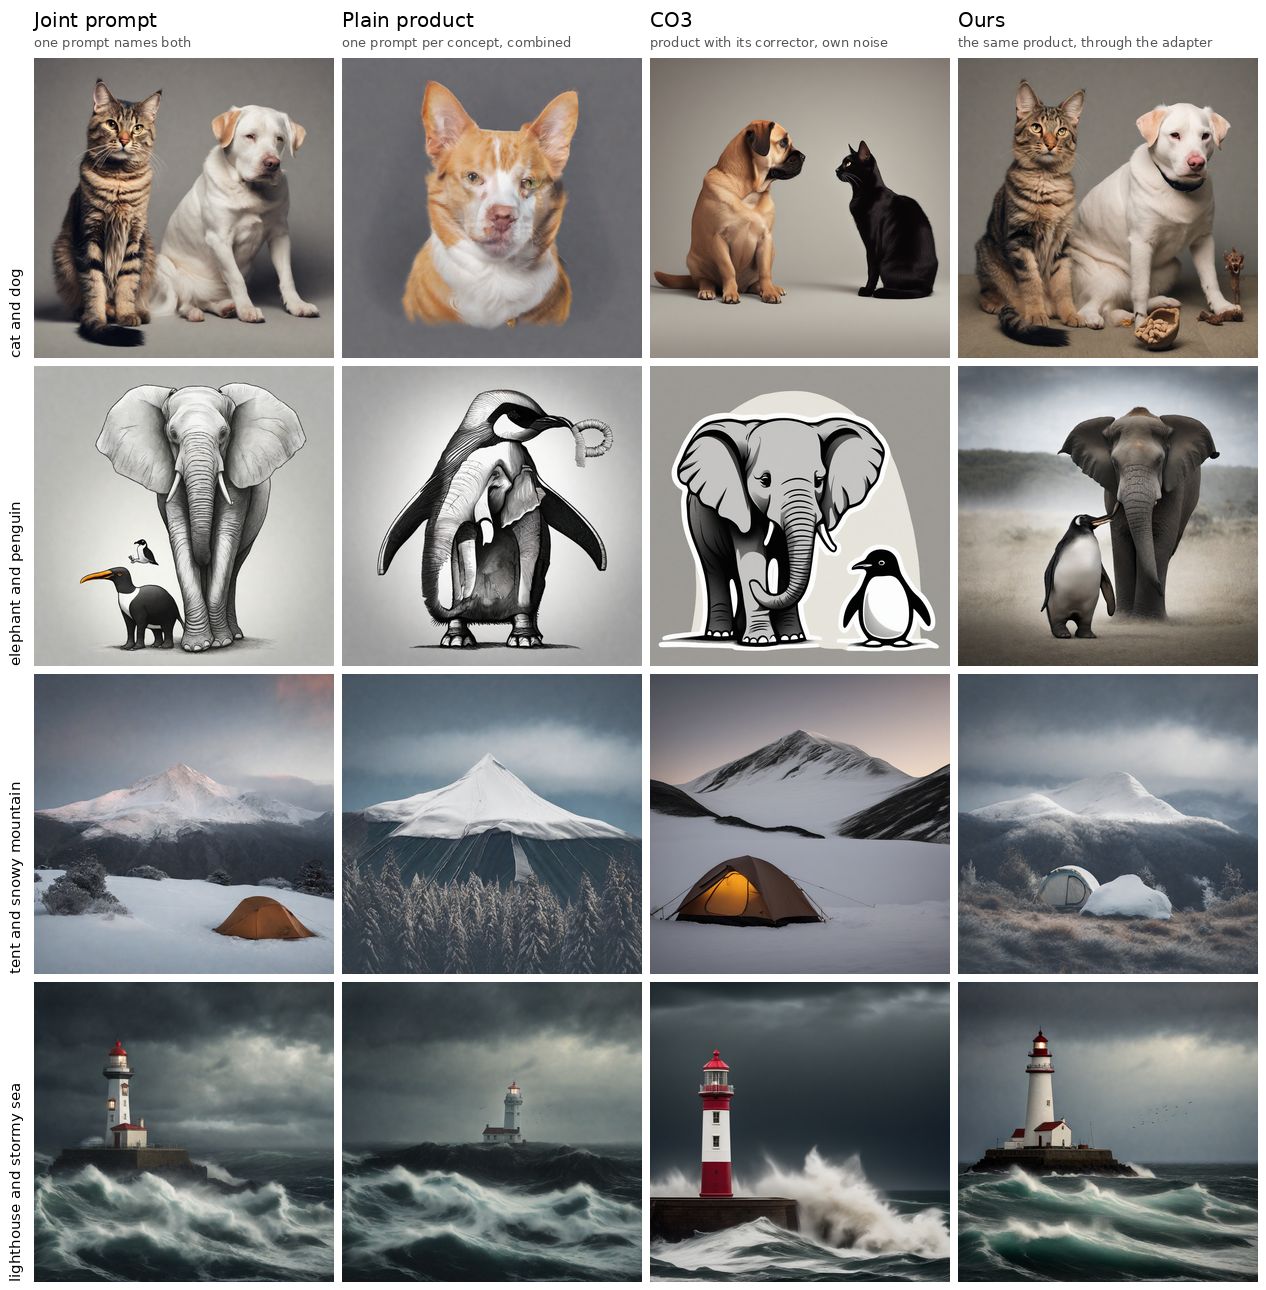
\includegraphics[width=0.544\textwidth,trim=34 932 0 40,clip]{four-pairs-four-methods.png} \\[-1pt]
% \rotatebox{90}{\scriptsize\makebox[0.1361\textwidth]{\shortstack{elephant and\\penguin}}} & 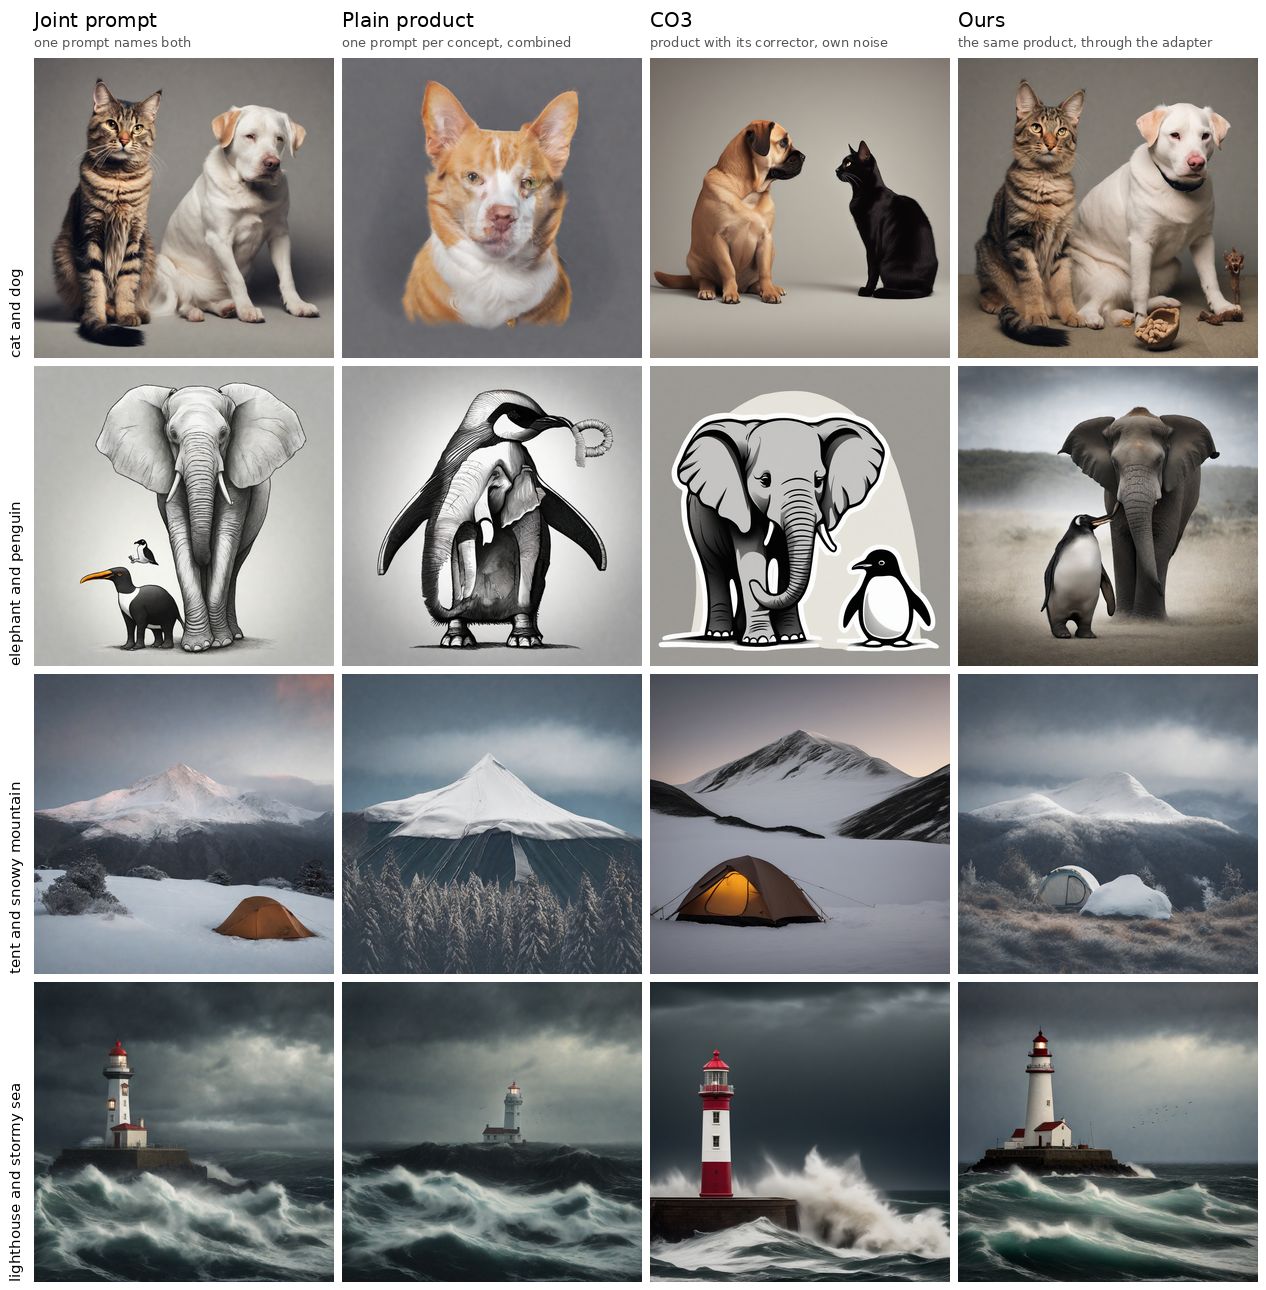
\includegraphics[width=0.544\textwidth,trim=34 624 0 348,clip]{four-pairs-four-methods.png} \\[-1pt]
% \rotatebox{90}{\scriptsize\makebox[0.1361\textwidth]{\shortstack{tent and\\snowy mountain}}} & 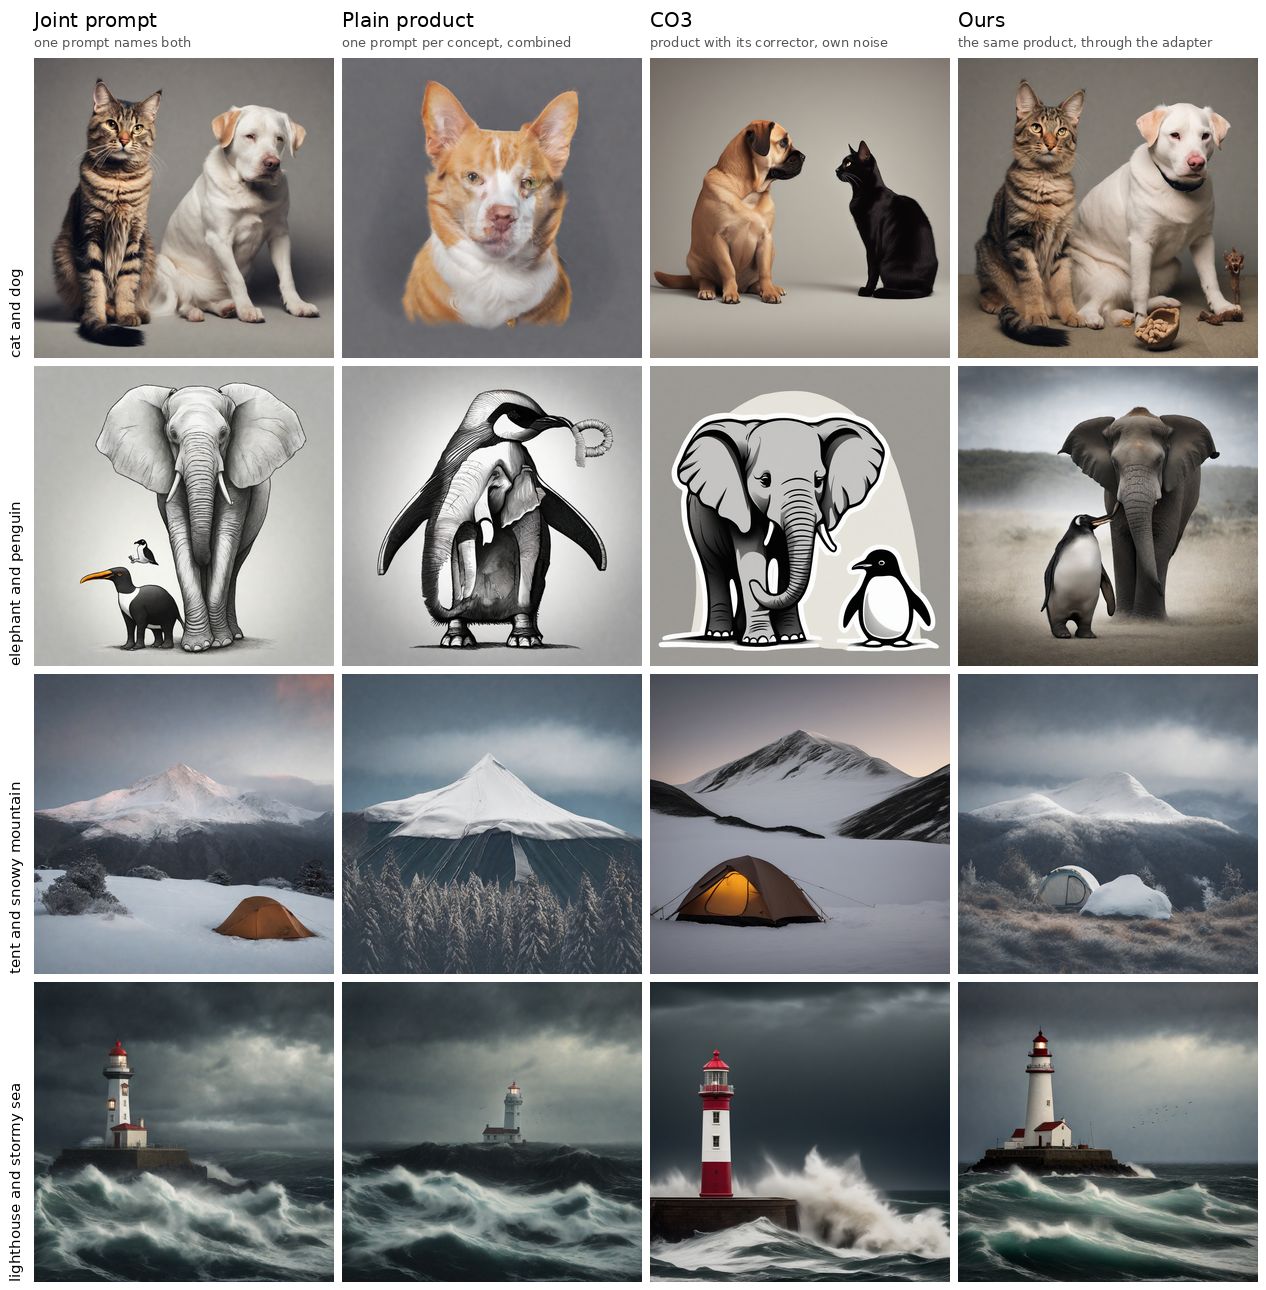
\includegraphics[width=0.544\textwidth,trim=34 316 0 656,clip]{four-pairs-four-methods.png} \\[-1pt]
% \rotatebox{90}{\scriptsize\makebox[0.1361\textwidth]{\shortstack{lighthouse and\\stormy sea}}} & 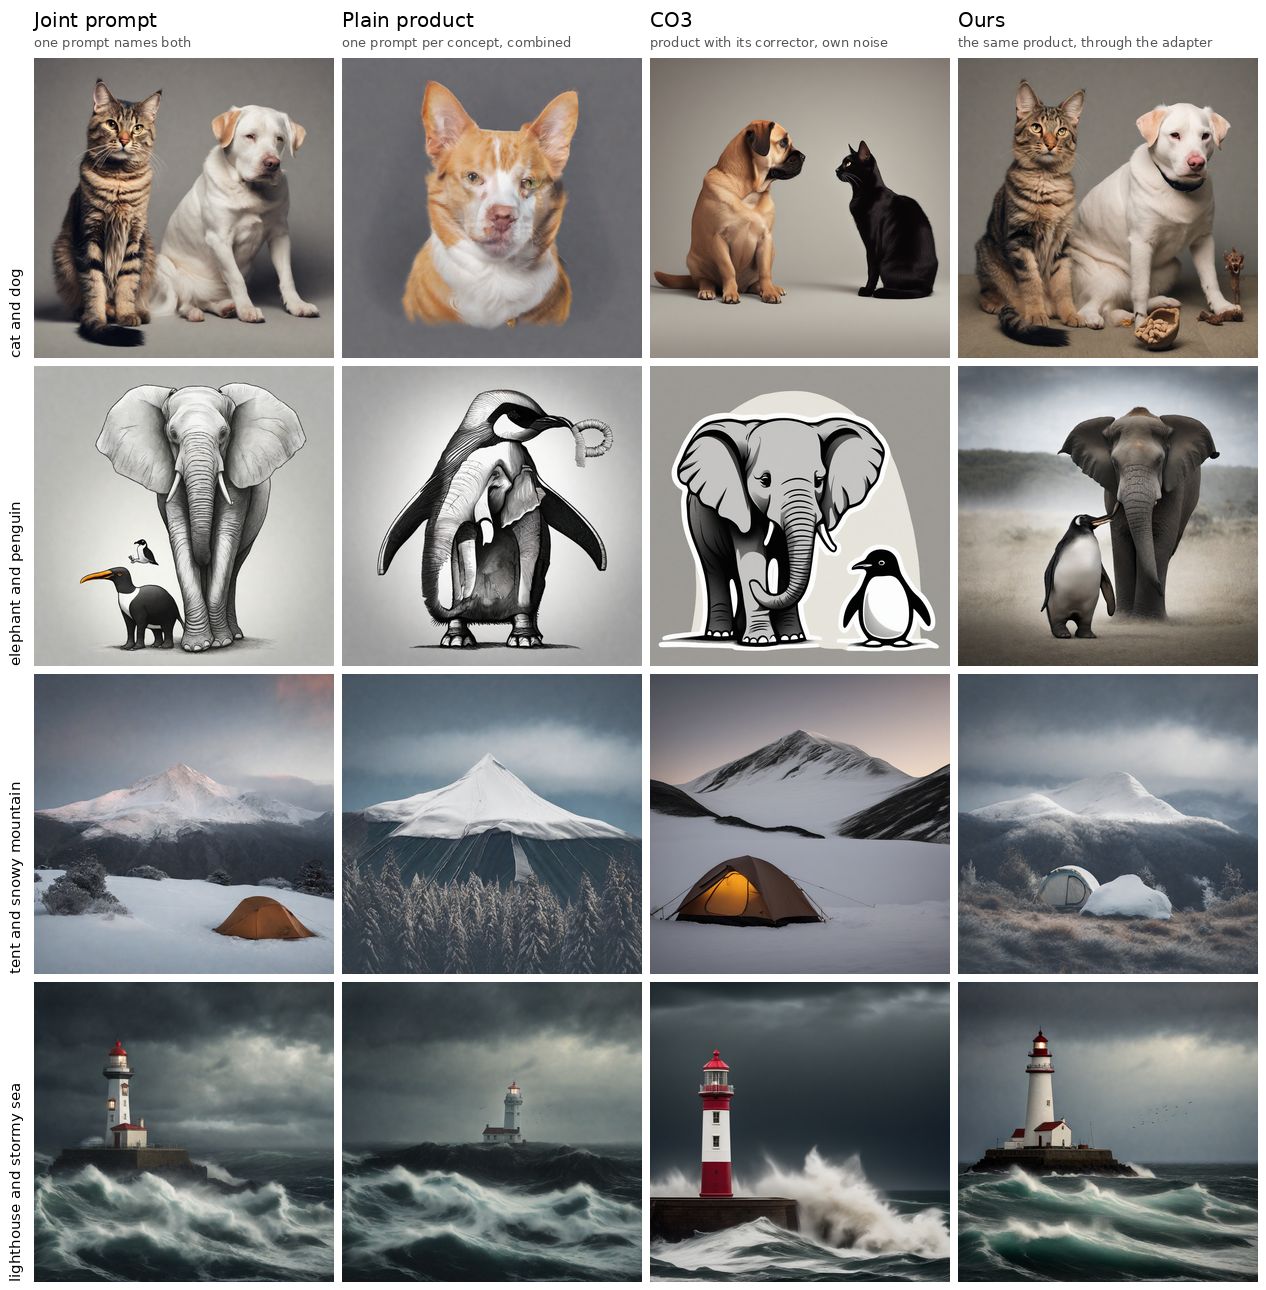
\includegraphics[width=0.544\textwidth,trim=34 8 0 964,clip]{four-pairs-four-methods.png} \\[-1pt]
% \end{tabular}
% \vspace{-4pt}
% \caption{\textbf{The adapter repairs the composition without the joint prompt.} Rows are four unseen concept pairs, and columns are the joint prompt, plain product, CO3, and our adapter. CO3 uses different starting noise; the other three columns share it.}
% \label{fig:four-pairs-four-methods}
% \vspace{-10pt}
% \end{wrapfigure}

Figure~\ref{fig:four-pairs-four-methods} shows the results of our method compared to joint prompting, PoE and CO3 (which still uses the joint prompt).  Importantly, for inference using our LoRA module the joint prompt is never evaluated, and inference still requires only three predictions per denoising step (one per concept and the null prompt where the LoRA is active within these predictions). As expected, joint prompting and CO3 show good performance for common pairs such as the lighthouse and sea which are likely to be explicitly in the Stable Diffusion XL training set. For uncommon pairs, even joint prompting can fail by including multiple legs on the penguin for example. CO3 correctly depicts a penguin and elephant separately, however completely changes the style to be a cartoon to accommodate this uncommon pairing. All columns start from the same latent. The second column shows the corresponding product-of-experts samples. In each case, the
two concepts are not preserved as distinct entities: the animals fuse, the tent and mountain
collapse into one cone-like shape. The lighthouse and sea appears structurally correct but the lighthouse itself is reduced to a distant object in the background. This reproduces the results of \citet{bradley2025mechanisms} which show that PoE will combine objects when they compete for the same position in an image and works reasonably well when there is a distinction between which objects should fall into the foreground and background. Finally, the LoRA module trained to restore plurality accurately does so across a range of different concepts. For the cat and dog it almost perfectly recovers the joint prompt (once again without ever having access to this joint prompt, where the consistency is due to the same seed and initial noise sample). For the uncommon pairing of the penguin and elephant it also accurately separate the objects. It is important to note that this pairing is a novel combination that the LoRA was not trained on as there are insufficient examples of a good joint prompt output for this pair (as shown by the failure of the joint prompt here). Thus, our LoRA module successful generalises and produces a structurally sound scene which composes distinct object at inference time.
% \begin{figure}[!htbp]
% \centering
% 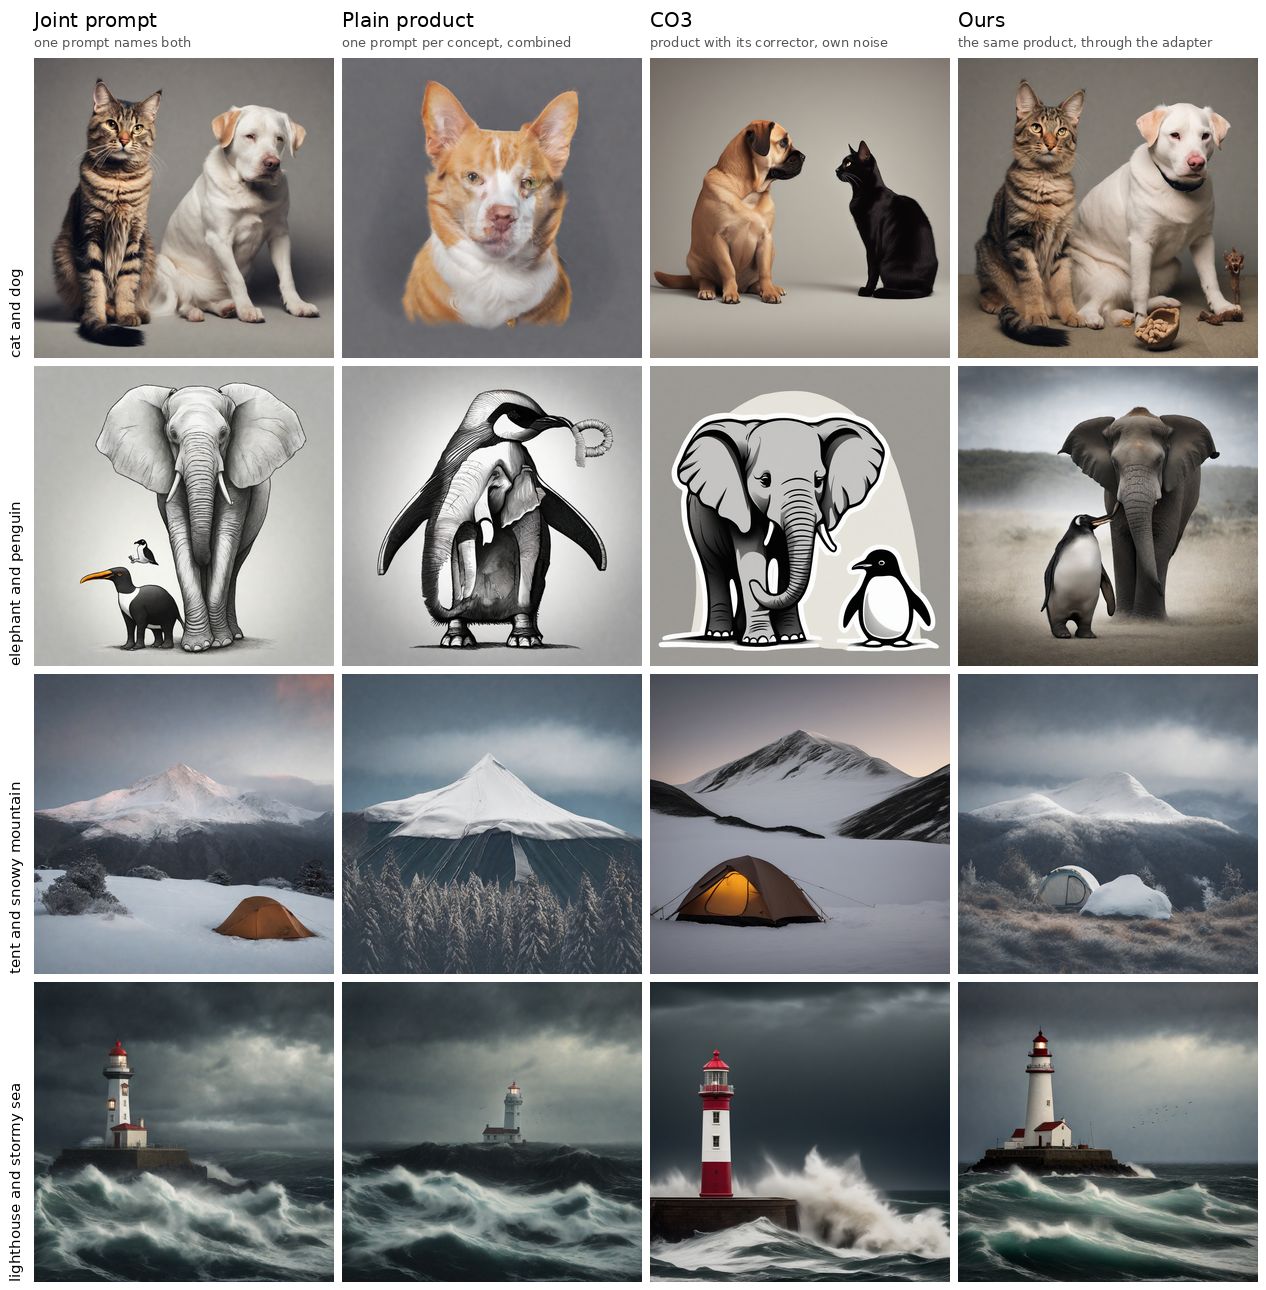
\includegraphics[width=0.72\textwidth]{four-pairs-four-methods.png}
% \caption{\textbf{The adapter repairs the composition without the joint prompt.} Rows are four unseen concept pairs, and columns are the joint prompt, plain product, CO3, and our adapter. CO3 uses different starting noise; the other three columns share it.}
% \label{fig:four-pairs-four-methods}
% \end{figure}


We also conduct a sensitivity analysis on the one hyper-parameter our method introduces, which is the rank of our LoRA module. Thus, we trained LoRA modules at different ranks to examine whether adapter capacity affects the recovery of two distinct animals. Figure~\ref{fig:adapter-rank} shows this comparison for ranks 8, 16, and 32. Each row uses the same sampled noise and seed. The rank-8 run produces heavily degraded images in which the cat and dog are largely lost in visual noise, while rank-16 and rank-32 runs produce two distinct animals. Thus, recovering plurality does require sufficient rank of the LoRA but beyond sufficient dimensionality performance remains consistent.
% \begin{figure}[!htbp]
% \centering
% \includegraphics[width=0.72\textwidth]{ablation/adapters-cat-dog-rank.png}
% \caption{\textbf{Cat--dog renders from different adapter rank runs.}
% Rows are held-out seeds 9, 11, and 12, with the same starting noise
% across each row. Columns show the plain product and adapters of rank 8,
% 16, and 32. The rank-8 run uses a later checkpoint than the rank-16
% and rank-32 runs.}
% \label{fig:adapter-rank}
% \end{figure}



% \begin{figure}[!htbp]
% \centering
% \includegraphics[width=\textwidth]{ablation/joint-prompt-through-adapter.png}
% \caption{\textbf{The adapter also changes joint-prompt renders.}
% Each row compares the model with and without the adapter under the
% same joint prompt and starting noise. Rows show a cat and a dog,
% a tiger and a dog, a chess board and an hourglass, and a picnic
% basket and a watermelon.}
% \label{fig:joint-prompt-through-adapter}
% \end{figure}


Finally, we report two limitation to our approach which should be noted and are demonstrated in Figure~\ref{fig:joint-prompt-through-adapter}. Firstly, we consider the effect of applying our LoRA module to a joint prompt. This test whether it can be applied to Stable Diffusion XL as a general property or if it should be used precisely during PoE. We see that the LoRA can change the output from joint prompting and it is not consistently better. For example, the cat and dog image is slightly corrupted and in the tiger and dog pairing it introduces a third animal which itself is a hybrid. However, in the case where the joint prompt fails such as the chessboard and hourglass the LoRA actually improved the image. For easy pairs it seems to have little impact on joint prompting, for example in the picnic basket and watermelon case. Thus, the LoRA module can introduce some instability during joint promting and should not be used for all image generations. Our LoRA-augmented PoE can also produce nonsensical which typically correspond to intrusion of new animals. For example, when prompted for a dog and a cat it produces a horse and a dog or a person with a dog. Another example introduces a third smaller cat into frame with a dog and a cat, showing that while the LoRA has learned plurality it is not necessarily counting. Finally, if the seed would typically produce a highly stylized image such as a line drawing or artwork the LoRA does not inject plurality. Thus, the LoRA is particularly useful for realistic styles where object positioning and scene structure is a more strict requirement. However, for styles where hybrid animals are more tolerable the LoRA sometimes does not change the final output.


% \begin{figure}[!htbp]
% \centering
% \includegraphics[width=0.72\textwidth]{how-a-render-fails-paper.png}
% \caption{\textbf{Five ways a corrected cat--dog render goes wrong.} The uncorrected hybrid (top left) is followed by five corrected failures: invented people, loss of semantic structure, a style change without separation, an extra animal, and the wrong species.}
% \label{fig:how-a-render-fails}
% \end{figure}

% TODO (ablations): Revisit this subsection when discussing training duration,
% held-out degradation, and checkpoint selection. Preserve these observations for
% the ablation discussion; assess the proposed trajectory-mismatch explanation
% against the evidence before restoring causal claims.
% \subsection{Where it breaks}
%
% Training the adapter is not stable. Past a point the held-out renders stop moving toward the
% joint-prompt image and start losing colour and detail, while the adapter's weights keep growing and
% the loss stays flat. The pairs it trained on never show this, so what decays is the generalisation we
% actually want, and there is no signal in the training loss that says when to stop. Part of the cause
% is in how the correction was collected. Every state the adapter learns from lies on an uncorrected
% run, but a corrected run leaves that trajectory at its first corrected step, so at inference the
% adapter is asked for a correction at states it never saw. That error enters the next step, and the
% run moves further from anything in its training data as it goes. The adapter also inherits what sits
% beneath it, since it corrects a product of two frozen experts and neither the failures of a single
% expert nor the failures of the product are its to fix. It supplies the missing plurality term and
% nothing else, which is why corrected renders still carry the ordinary mistakes of the model
% underneath.

% \FloatBarrier
\FloatBarrier
\section{Discussion}
\label{sec:conclusion}
In this work we introduce the concept of plurality: the notion that distinct objects in a prompts should become distinct objects in a generated image. We show that PoE and similar compositional diffusion methods are unable to create images with plurality, and instead create hybrid objects that combine the individual objects being prompted for. We show that plurality can be restored during early denoising with PoE and train a LoRA module to supply this correction while keeping a base Stable Diffusion XL model frozen. Crucially, the adapter restores composition on concept pairs unseen during training, using only the separate concept prompts and the null token at inference which are needed for PoE. Consequently, by using a finite set of easily obtained examples where joint prompting demonstrates plurality we can train a LoRA to apply the concept more broadly. Thus, our method is able to achieve the coherent image generation of joint prompting without the need for large quantities of data and exhaustive examples of concept pairs.

\looseness=-1
This work identifies a more general principle: the fact that written text often has implied information which can be learned and encoded by text-to-image generation models. Fundamentally, this is the core result of Section~\ref{Measuring} which shows that a joint prompt such as ``a cat and a dog'' not only encodes the objects which are desire (the cat and the dog independently) but implies a spatial relation between them. When a compositional diffusion method is used to separate the prompt into ``a cat'' and ``a dog'' neither individual prompt contains the same implication -- neither prompt encodes a restriction on the positioning of the object as, from the perspective of each prompt, there is only one object. While we have focused on plurality in this work, it is plausible that many more joint prompts can be identified with new examples of implied concepts. Our work here provides a framework for measuring and distilling these concepts into a module which can then be used to augment compositional diffusion in a principled manner. Thus, we take a step towards diffusion which can efficiently compose objects at inference time.


\section{AI Declaration}
In this work we made use of generative AI tools for coding assistance, to polish writing, retrieval of papers and generation of figures. We have not used AI for any other tasks. All AI assisted work was reviewed and manually tested. We take responsibility for the final content of this work, including text, claims or artifacts produced with the aid of generative AI.

% \section*{Ethics Statement}

% Lorem ipsum dolor sit amet, consectetur adipiscing elit. Integer tincidunt. Cras dapibus; vivamus elementum semper nisi. This placeholder should eventually discuss possible misuse, sensitive data, evaluation harms, environmental cost, or deployment constraints.

% \section*{Reproducibility Statement}

% Lorem ipsum dolor sit amet, consectetur adipiscing elit. Praesent congue erat at massa. Sed cursus turpis vitae tortor. This placeholder should eventually list code release status, random seeds, hardware, dataset provenance, hyperparameters, and any withheld artifacts.

% \section*{Acknowledgments}

% This anonymous placeholder contains no acknowledgments for submission. Replace this paragraph or remove the section for the initial blind review version if needed.

\bibliography{iclr2027_conference}
\bibliographystyle{iclr2027_conference}

% \appendix

% \section{Extended Related Work}
% \label{app:related}

% \subsection{Additional adaptation literature}

% Lorem ipsum dolor sit amet, consectetuer adipiscing elit. Aenean commodo ligula eget dolor. Aenean massa. Donec quam felis, ultricies nec, pellentesque eu, pretium quis, sem. This appendix slot is for adjacent methods that matter but would slow the main narrative.

% \subsection{Additional benchmarking literature}

% Nulla consequat massa quis enim. Donec pede justo, fringilla vel, aliquet nec, vulputate eget, arcu. In enim justo, rhoncus ut, imperdiet a, venenatis vitae, justo. This paragraph can become a longer comparison of benchmarks, threat models, and evaluation protocols.

% \subsection{Additional generation or exploration literature}

% Nullam dictum felis eu pede mollis pretium. Integer tincidunt. Cras dapibus; vivamus elementum semper nisi. Aenean vulputate eleifend tellus. This paragraph can become a longer bridge to diffusion models, search procedures, exploration policies, or sample generators.

% \section{Additional Method Details}
% \label{app:method-details}

% \subsection{Derivation of the product form and the plurality factor}
% \label{app:poe-derivation}

% Product-of-experts composition is obtained as follows \citep{liu2022compositional}.

% \begin{align}
% p(x \mid c_1, c_2)
%   &\propto p(x)\, p(c_1 \mid x)\, p(c_2 \mid x) \label{eq:independence}\\
%   &= p(x) \cdot \frac{p(x \mid c_1)\, p(c_1)}{p(x)} \cdot \frac{p(x \mid c_2)\, p(c_2)}{p(x)} \\
%   &= p(c_1)\, p(c_2) \cdot \frac{p(x \mid c_1)\, p(x \mid c_2)}{p(x)} \\
%   &\propto \frac{p(x \mid c_1)\, p(x \mid c_2)}{p(x)}
% \end{align}

% The unconditional density is in the denominator because it is already contained in both conditional experts, so their product carries it twice and one copy has to be removed.

% The gap between the joint conditional and the product form can be written as

% \begin{align}
% R_t &\;\equiv\; \frac{p(c_1, c_2 \mid x_t)}{p(c_1 \mid x_t)\, p(c_2 \mid x_t)}\\
% p(c_1, c_2 \mid x_t) &= p(c_1 \mid x_t)\, p(c_2 \mid x_t)\, R_t
% \end{align}

% $R_t$ equals one exactly when the two concepts are independent given the state. Carrying it through the same Bayes steps recovers the joint conditional from the product form.

% \begin{align}
% p(x_t \mid c_1, c_2)
%   &\propto p(x_t)\, p(c_1, c_2 \mid x_t) \\
%   &= p(x_t)\, p(c_1 \mid x_t)\, p(c_2 \mid x_t)\, R_t \\
%   &\propto p(x_t)\, \frac{p(x_t \mid c_1)}{p(x_t)}\, \frac{p(x_t \mid c_2)}{p(x_t)}\, R_t
%   &&\text{(Bayes on each factor, as in \eqref{eq:independence})}\\
%   &\propto \frac{p(x_t \mid c_1)\, p(x_t \mid c_2)}{p(x_t)}\, R_t \\
%   &\propto p_{\mathrm{PoE}}(x_t \mid c_1, c_2)\, R_t
% \end{align}

% Taking the gradient of the logarithm of both sides, and converting scores to noise predictions, gives the relation between the true joint prediction and the product-of-experts prediction stated in Section~\ref{sec:interaction}.

% \subsection{Derivation of the placeholder objective}

% Lorem ipsum dolor sit amet, consectetur adipiscing elit. Let $\theta^{\star}$ denote the best adapted parameter under the placeholder score:
% \begin{equation}
%     \theta^{\star}
%     =
%     \argmin_{\theta'}
%     \left[
%     \mathcal{L}(\theta')
%     +
%     \eta
%     \left\|
%     \nabla_{\theta'} \mathcal{L}(\theta')
%     \right\|_{2}^{2}
%     \right].
%     \label{eq:appendix-objective}
% \end{equation}
% Sed ut perspiciatis unde omnis iste natus error sit voluptatem accusantium doloremque laudantium. Replace this derivation with the real loss, estimator, theorem, or convergence argument.

% \subsection{Placeholder proposition}

% \newtheorem{proposition}{Proposition}
% \begin{proposition}[Placeholder stability]
% Assume the score in Eq.~\ref{eq:score} is $L$-Lipschitz in $\theta'$ and that the adaptation operator in Eq.~\ref{eq:adaptation} changes by at most $\epsilon$ under a single-regime perturbation. Then the reported score changes by at most $L\epsilon$.
% \end{proposition}

% \paragraph{Proof sketch.}
% Lorem ipsum dolor sit amet, consectetur adipiscing elit. By the Lipschitz assumption,
% \begin{equation}
%     \left|S(\theta'_{a},\mathcal{D}_{2}) - S(\theta'_{b},\mathcal{D}_{2})\right|
%     \leq
%     L\left\|\theta'_{a}-\theta'_{b}\right\|_{2}
%     \leq
%     L\epsilon.
% \end{equation}
% Quisque rutrum aenean imperdiet. Etiam ultricies nisi vel augue. Replace this proof sketch with the real theorem or delete it if the paper is purely empirical.

% \subsection{Implementation notes}

% Suspendisse potenti. Sed lectus. Integer euismod lacus luctus magna. Quisque cursus, metus vitae pharetra auctor, sem massa mattis sem, at interdum magna augue eget diam. Use this subsection for architecture details, preprocessing choices, batching, optimizer settings, and implementation deviations from prior work.

% \section{Additional Experimental Results}
% \label{app:additional-results}

% \subsection{Full metric matrix}

% Lorem ipsum dolor sit amet, consectetur adipiscing elit. Phasellus viverra nulla ut metus varius laoreet. Table~\ref{tab:full-matrix} is a fake expanded result table for all regimes and metrics.

% \begin{table}[h]
% \caption{Placeholder full metric matrix}
% \label{tab:full-matrix}
% \begin{center}
% \begin{tabular}{lcccccc}
% \hline
% \textbf{Method} & \textbf{U1} & \textbf{U2} & \textbf{R1} & \textbf{R2} & \textbf{C1} & \textbf{C2} \\
% \hline
% Baseline A & 71.2 & 68.9 & 22.4 & 19.5 & 1.00 & 0.82 \\
% Baseline B & 73.5 & 69.4 & 20.1 & 18.7 & 1.18 & 0.79 \\
% \methodname & 78.9 & 75.6 & 16.3 & 14.2 & 1.09 & 0.76 \\
% Oracle & 82.0 & 78.2 & 12.0 & 10.5 & 2.40 & 0.64 \\
% \hline
% \end{tabular}
% \end{center}
% \end{table}

% \subsection{Additional curves}

% Morbi nec metus. Phasellus blandit leo ut odio. Maecenas ullamcorper, dui et placerat feugiat, eros pede varius nisi, condimentum viverra felis nunc et lorem. Figure~\ref{fig:appendix-curves} is reserved for secondary sweeps or per-domain curves.

% \begin{figure}[h]
% \placeholderfigure{1.75in}{Appendix curves}
% \caption{Placeholder appendix curves. Replace with per-domain plots, seed-level traces, or confidence intervals.}
% \label{fig:appendix-curves}
% \end{figure}

% \subsection{Qualitative examples}

% Donec vitae sapien ut libero venenatis faucibus. Nullam quis ante. Etiam sit amet orci eget eros faucibus tincidunt. This subsection can hold generated samples, rollouts, extracted examples, failure cases, or visual inspection panels.

% \begin{figure}[h]
% \placeholderfigure{1.85in}{Qualitative examples}
% \caption{Placeholder qualitative examples. Replace with representative successes and failures, not only favorable cases.}
% \label{fig:qualitative}
% \end{figure}

% \section{Experimental Details}
% \label{app:experimental-details}

% \subsection{Datasets, domains, and splits}

% Lorem ipsum dolor sit amet, consectetur adipiscing elit. Vestibulum ullamcorper mauris at ligula. Fusce fermentum odio nec arcu. Table~\ref{tab:hyperparameters} is a placeholder for reproducibility-critical settings.

% \begin{table}[h]
% \caption{Placeholder hyperparameters}
% \label{tab:hyperparameters}
% \begin{center}
% \begin{tabular}{ll}
% \hline
% \textbf{Setting} & \textbf{Value} \\
% \hline
% Batch size & 128 \\
% Learning rate & $3 \times 10^{-4}$ \\
% Training steps & 100,000 \\
% Evaluation seeds & 10 \\
% Selection metric & Validation score \\
% Hardware & Placeholder accelerator \\
% \hline
% \end{tabular}
% \end{center}
% \end{table}

% \subsection{Baselines and implementations}

% Pellentesque auctor neque nec urna. Proin sapien ipsum, porta a, auctor quis, euismod ut, mi. Aenean viverra rhoncus pede. Replace this with exact baseline names, official repositories, commit hashes, and any local modifications.

% \subsection{Compute resources}

% Vivamus elementum semper nisi. Aenean vulputate eleifend tellus. Aenean leo ligula, porttitor eu, consequat vitae, eleifend ac, enim. Replace this with accelerator type, wall-clock cost, memory footprint, and total experiment budget.

% \section{Limitations, Broader Impact, and LLM Use}
% \label{app:limitations}

% \subsection{Limitations}

% Lorem ipsum dolor sit amet, consectetur adipiscing elit. Suspendisse enim turpis, dictum sed, iaculis a, condimentum nec, nisi. Praesent nec nisl a purus blandit viverra. Replace this with the strongest known caveats, including assumptions that future reviewers are likely to probe.

% \subsection{Broader impact}

% Nullam vel sem. Nam ipsum risus, rutrum vitae, vestibulum eu, molestie vel, lacus. Sed magna purus, fermentum eu, tincidunt eu, varius ut, felis. Replace this with a domain-specific risk and benefit analysis.

% \subsection{Use of large language models}

% In the preparation of this placeholder manuscript, language models may be used for drafting filler, refactoring prose, and checking consistency. Replace this statement with the final, accurate disclosure for the submitted paper.


% Keep the appendix separate from the bibliography and earlier floats.
\clearpage
\appendix
% The appendix holds stacks of tables and image grids; let a page carry several of them.
\setcounter{topnumber}{3}\setcounter{bottomnumber}{2}\setcounter{totalnumber}{4}\renewcommand{\textfraction}{0.07}




\section{Implementation details}
\label{app:implementation}

Every run samples with 50 DDIM steps at guidance weight 7.5, at $1024\times1024$ resolution, in fp16. The adapter has rank \adrank{} with $\alpha = r$, so its update is added at full scale. It adds \adparams{}\,M trainable parameters to the \adbase{}\,B-parameter frozen base. We train it with AdamW on a schedule of 50{,}000 optimizer steps (1{,}000 epochs of 50); the learning rate starts at $10^{-4}$ and follows a cosine schedule that reaches zero at the end. We use the checkpoint at \adsteps{} steps (\adepochs{} epochs). Gradients are clipped at norm 1.0. 

\paragraph{Training pairs.} The adapter trains on \trainpairs{} pairs. Each training cell is one pair at one seed, and its target is the picture the joint prompt draws on that seed, never CO3's. Pairs were admitted over several rounds in which a person judged whether the joint prompt draws both named things; not every kept seed was checked on its own, and a few targets show only one of the two. Twenty-eight pairs are two animals (horse and pig, lion and meerkat, donkey and duck), three are an animal and an object (hamster and carrot, pony and red barn, snail and lantern), and seventeen are two objects (lighthouse and sailboat, microscope and test tube, windmill and tractor). Training uses 182 cells over 23 seeds, seeds 1 to 8 and 17 upward; seeds 9 to 16 are never trained on, because the cached starting noise is shared across pairs and they are the evaluation seeds. Figure~\ref{fig:training-examples} shows the target for nine of them, three of each kind. The full list is released with the code as the configuration file it reads.

\begin{figure}[htbp]
\centering
\includegraphics[width=\textwidth]{ablation/training-target-examples.pdf}
\caption{\textbf{Examples of training targets.} The joint prompt's picture for nine of the \trainpairs{} training pairs, one kept seed each, grouped by the kind of pair. The adapter learns to reproduce these pictures from the separate concept prompts.}
\label{fig:training-examples}
\end{figure}

\begin{figure}[htbp]
\centering
\includegraphics[width=\textwidth]{ablation/joint-prompt-screening.pdf}
\caption{\textbf{Screening candidate pairs with the joint prompt and CO3.} Each seed shows the joint prompt's picture (left) and CO3's (right). A green frame marks, for each seed, the picture that shows the two named animals as separate animals most clearly. Crow and raven was dropped because the two birds are hard to tell apart (red frames).}
\label{fig:training-choice}
\end{figure}

% Hidden 2026-11-11 until the CO3 pair filter is settled; restore the figure and the sentence below together.
% Figure~\ref{fig:training-selection} sets the joint prompt beside CO3 for five candidate pairs at seeds 1 to 3. Horse and pig, lion and meerkat, and gorilla and chimpanzee are in the pool on all three seeds, including gorilla and chimpanzee's seed 1, where the joint prompt draws two gorillas; crow and raven was left out because the two birds cannot be told apart, and giraffe and hippo was left out as well. CO3 draws both animals about as often, sometimes in an illustrated style, but none of its pictures is used as a target. 
% \begin{figure}[htbp]
% \centering
% \includegraphics[width=\textwidth]{ablation/joint-prompt-beside-co3.pdf}
% \caption{\textbf{The joint prompt beside CO3 on five candidate pairs.} Each seed shows the joint prompt's picture on the left and CO3's on the right; CO3 starts from its own noise. A green frame marks a picture used as a training target; no CO3 picture is one. A red frame marks a seed where neither picture shows the two named animals as different animals.}
% \label{fig:training-selection}
% \end{figure}

% Hidden until the diagram uses the paper's notation (Equation 12, \hat\epsilon, c_1).
% Figure~\ref{fig:adapter-training} shows how these runs are trained. Frozen SDXL first supplies the joint-prompt target on states cached from a plain product-of-experts trajectory. At each selected state, the adapted network evaluates the two concept prompts and the null token separately; their composed prediction is compared with that target. The loss updates only the LoRA weights. The diagram separates the one-time target cache from the three adapted predictions and the loss used to update the LoRA weights.

% \begin{figure}[!htbp]
% \centering
% \includegraphics[width=\textwidth,trim=10bp 110bp 10bp 85bp,clip]{training-the-compositional-adapter.jpg}
% \caption{\textbf{Training the compositional adapter.} A cached frozen joint-prompt target supervises the adapted product-of-experts prediction; only the LoRA weights are updated. The frozen network supplies the cached target; the adapted network produces the composition matched to it.}
% \label{fig:adapter-training}
% \end{figure}
\FloatBarrier

% Retained for later revision; excluded from the current paper.
% \section{The loss weight}
% \label{app:loss-weight}
%
% Inverting \eqref{eq:forward} turns a noise prediction into an estimate of the clean latent,
% $\hat x_0(\epsilon) = (x_t - \sqrt{1-\bar\alpha_t}\,\epsilon)/\sqrt{\bar\alpha_t}$. Two such
% estimates formed from the same $x_t$ differ by $\sqrt{1-\bar\alpha_t}/\sqrt{\bar\alpha_t}$ times the
% difference of the predictions, so scaling a squared error in noise space by
% $(1-\bar\alpha_t)/\bar\alpha_t$ gives the squared error on the clean latent. This is a weighting over
% noise levels in the sense of \citet{kingma2023understanding}, and the reason for preferring the
% clean-latent distance is the one \citet{li2025basics} give: clean data and noised quantities are
% different prediction problems.
%
% On SDXL's schedule over the 50-step DDIM grid, that factor runs from 172 at the first step to 0.002
% at the last, so the first step alone would take most of the gradient. We clamp it at
% $\kappa = \lossclamp$ and divide by the mean of the clamped factor over the grid, $Z = \lossnorm$,
% which keeps the loss scale comparable to the unweighted objective:
% \begin{equation}
% \gamma_t = \frac{1}{Z}\,\min\!\left(\frac{1-\bar\alpha_t}{\bar\alpha_t},\ \kappa\right).
% \label{eq:loss-weight}
% \end{equation}
%
% Written on the noise-space loss, this is the Min-SNR weighting of \citet{hang2023efficient} with
% their clamp set to $1/\kappa \approx 0.045$ instead of their default of 5. The clamp binds through
% step 10, so $\gamma_t$ is constant at $2.96$ over the first eleven steps and falls to
% $2.3\times10^{-4}$ by step 49. Two consequences follow. Where the clamp binds the weight is flat, so
% over those eleven steps the objective is the noise-space distance rather than the clean-latent one.
% And those eleven steps are the window Section~\ref{sec:analysis} found decisive, so the objective
% concentrates on that window by construction rather than by discovery.
%
% All three values depend on the schedule and the step count: changing the number of denoising steps
% moves $\kappa$'s binding point, $Z$, and the range of the raw factor.

\section{Training and inference derivation}
\label{app:training-inference}

The base network has frozen parameters $\theta$; only the LoRA parameters $\psi$ change during
training. We use $c_1=\text{``a cat''}$ and $c_2=\text{``a dog''}$ as an example, write
$c_{12}=\text{``a cat and a dog''}$ for the joint prompt, and denote the null token by
$\emptyset$. Every prediction below is evaluated at the same noisy latent $x_t$ and timestep $t$.

\subsection{Composing the adapted predictions}

The adapter never receives $c_{12}$. It receives $c_1$, $c_2$, and $\emptyset$ in three
separate forward passes, producing
\begin{equation}
\begin{aligned}
a_\psi &= \epsilon_{\theta,\psi}(x_t,t\mid c_1), &
 b_\psi &= \epsilon_{\theta,\psi}(x_t,t\mid c_2), &
 u_\psi &= \epsilon_{\theta,\psi}(x_t,t\mid\emptyset).
\end{aligned}
\label{eq:adapted-predictions}
\end{equation}
With classifier-free guidance weight $w$, each concept prediction is guided against the same
null prediction: $g_1=u_\psi+w(a_\psi-u_\psi)$ and
$g_2=u_\psi+w(b_\psi-u_\psi)$. Adding the two guided predictions counts the shared null
prediction twice, so one copy is subtracted:
\begin{align}
\hat\epsilon^{\psi}_{\mathrm{PoE}}
 &= g_1+g_2-u_\psi \nonumber\\
 &= u_\psi+w(a_\psi-u_\psi)+w(b_\psi-u_\psi) \nonumber\\
 &= u_\psi+w(a_\psi+b_\psi-2u_\psi).
\label{eq:adapted-poe}
\end{align}
At $w=1$, this is $a_\psi+b_\psi-u_\psi$; the runs in this paper use $w=7.5$.

\subsection{From the training target to inference}

For comparison, write the frozen network's three separate predictions as
$a_0=\epsilon_\theta(x_t,t\mid c_1)$, $b_0=\epsilon_\theta(x_t,t\mid c_2)$, and
$u_0=\epsilon_\theta(x_t,t\mid\emptyset)$. Its product-of-experts prediction is
\begin{equation}
\hat\epsilon_{\mathrm{PoE}}=u_0+w(a_0+b_0-2u_0).
\end{equation}
The frozen network also evaluates the joint prompt during training. Writing
$j_0=\epsilon_\theta(x_t,t\mid c_{12})$, its guided joint-prompt target is
\begin{equation}
\hat\epsilon_{\mathrm{Mono}}=u_0+w(j_0-u_0).
\end{equation}
The plurality term is the difference between these two frozen predictions at the same state:
\begin{equation}
r_t=\hat\epsilon_{\mathrm{Mono}}-\hat\epsilon_{\mathrm{PoE}},
\qquad
\hat\epsilon_{\mathrm{Mono}}=\hat\epsilon_{\mathrm{PoE}}+r_t.
\end{equation}
Training matches the adapted composition to the frozen joint-prompt target. Consequently,
$\hat\epsilon^{\psi}_{\mathrm{PoE}}\approx\hat\epsilon_{\mathrm{PoE}}+r_t$ on the
training states. Defining the change made by the adapter as
\begin{equation}
\hat r_\psi
  =\hat\epsilon^{\psi}_{\mathrm{PoE}}-\hat\epsilon_{\mathrm{PoE}},
\qquad
\hat\epsilon^{\psi}_{\mathrm{PoE}}
  =\hat\epsilon_{\mathrm{PoE}}+\hat r_\psi,
\end{equation}
shows what training asks it to supply: $\hat r_\psi\approx r_t$. The equality in the
second expression is exact by definition; the approximation depends on how well the adapter
matches the target. The early denoising steps are where this agreement matters most for
composition.

At inference, sampling starts from $x_T\sim\mathcal N(0,I)$ and evaluates only $c_1$,
$c_2$, and $\emptyset$ at each step. Their adapted predictions give
$\hat\epsilon^{\psi}_{\mathrm{PoE}}$ directly, without evaluating $c_{12}$. The
joint-prompt target supplies supervision during training, while sampling retains the same
three prompt evaluations per step as ordinary product-of-experts composition.

% \section{The strength sweep and its controls}
% \label{app:strength-sweep}

% room for this section's first float, so its heading never sits alone at a page foot
\Needspace{6.4in}
\section{Review response material}
\label{app:review-slots}

\subsection{The benchmark prompts}
\label{app:review-benchmarks}

Table~\ref{tab:review-R1} scores every method on the 276 Attend-and-Excite prompts (66 animal pairs, 144 animal-object pairs, 66 object pairs) at seeds 9 to 12. Figure~\ref{fig:review-R12} shows two prompts from each set at seed 9, every method from the same starting noise. Table~\ref{tab:review-R14} adds GenEval's two-object and counting tasks and T2I-CompBench's spatial and complex tasks, each scored by its official evaluator on its own prompts.

\begin{figure}[htbp]
\centering\footnotesize
\reviewslot{R12}{\linewidth}{5.2in}
\caption{\textbf{The images behind Table~\ref{tab:review-R1}.} Two prompts from each set at seed 9; columns are the methods of Table~\ref{tab:review-R1} in its order.}
\label{fig:review-R12}
\end{figure}

\begin{table}[htbp]
\centering\footnotesize
\caption{\textbf{Standard benchmarks on their own prompts with SDXL.} GenEval's two-object and counting tasks and T2I-CompBench's spatial and complex tasks, each scored by its official evaluator; higher is better. NFE as in Table~\ref{tab:review-R1}.}
\label{tab:review-R14}
\smallskip
\reviewslot{R14}{\linewidth}{1.6in}
\end{table}
\FloatBarrier

% room for this subsection's first float, so its heading never sits alone at a page foot
\Needspace{5.8in}
\subsection{The held-out pairs}
\label{app:review-held-out}

Table~\ref{tab:review-R3} groups the 53 held-out pairs by whether the joint prompt composes them: hard, easy but unseen, and not competing. None of these pairs was trained on as a pair, but 30 of the 53 share a concept with a training pair (cow and horse shares the horse of horse and pig), and 6 share both concepts, each with a different training pair. Figure~\ref{fig:review-R4} shows one pair per group at seeds 9 and 10, and the list below names every pair.

\begin{figure}[htbp]
\centering\footnotesize
\reviewslot{R4}{\linewidth}{5.0in}
\caption{\textbf{The images behind Table~\ref{tab:review-R3}.} One pair from each group at seeds 9 and 10; columns are the methods of Table~\ref{tab:review-R3} in its order, each from the same starting noise.}
\label{fig:review-R4}
\end{figure}

\paragraph{Pairs used in evaluation.} The 53 held-out pairs by group, and the two pairs used to choose the adapter. The number after a pair is the seeds out of 8 on which the joint prompt shows both named things; $^*$marks a pair held out when the adapter was trained.
\label{sec:review-R7}

\reviewslot{R7}{\linewidth}{1.6in}
\FloatBarrier

% room for this subsection's first float, so its heading never sits alone at a page foot
\Needspace{2.8in}
\subsection{Stable Diffusion 1.5}
\label{app:review-sd15}

Attend-and-Excite, SynGen and Divide-and-Bind are released for Stable Diffusion 1.x only, so Table~\ref{tab:review-R5} runs them from their official code on the same prompts. Its numbers compare only within the table, because the base model differs from Table~\ref{tab:review-R1}'s. Figure~\ref{fig:review-R13} shows the prompts of Figure~\ref{fig:review-R12} under these methods.

\begin{table}[htbp]
\centering\footnotesize
\caption{\textbf{The Attend-and-Excite prompts with SD 1.5.} Columns as in Table~\ref{tab:review-R1}. SD 1.5 methods run from their official code, which targets SD 1.x; a number compares only within its table.}
\label{tab:review-R5}
\smallskip
\reviewslot{R5}{\linewidth}{1.8in}
\end{table}

\begin{figure}[htbp]
\centering\footnotesize
\reviewslot{R13}{\linewidth}{3.6in}
\caption{\textbf{The images behind Table~\ref{tab:review-R5}.} The prompts of Figure~\ref{fig:review-R12} with the SD 1.5 methods of Table~\ref{tab:review-R5}.}
\label{fig:review-R13}
\end{figure}
\FloatBarrier

% room for this subsection's first float, so its heading never sits alone at a page foot
\Needspace{4.4in}
\subsection{How the adapter behaves}
\label{app:review-adapter}

Figure~\ref{fig:adapter-rank} varies the adapter's rank and the number of denoising steps it acts on, for a cat and a dog at three held-out seeds; Section~\ref{sec:results} discusses it. Figure~\ref{fig:review-R9} counts each failure type over the held-out pairs as the adapter acts on fewer steps, and Figure~\ref{fig:review-R10} shows the images behind those counts.

\begin{figure}[htbp]
\centering
\includegraphics[width=\textwidth]{ablation/adapter-settings-full-width.pdf}
\caption{\textbf{Effect of adapter settings on composing a cat and a dog.}
Each row uses one held-out seed and the same starting noise across
columns. The left group compares the uncorrected product with adapters
of rank 8, 16, and 32. The right group compares correction during the
first 10, first 25, or all 50 denoising steps. After the adapter stops, the PoE completes the remaining steps. Therefore, the first column of the right groups shows the adapter acting on the 10 steps followed by 40 steps of uncorrected composition.}
\label{fig:adapter-rank}
\end{figure}



\begin{figure}[htbp]
\centering\footnotesize
\reviewslot{R9}{\linewidth}{2.0in}
\caption{\textbf{Failure types as the adapter acts on fewer steps.} Counts of each failure type over the held-out pairs with no adapter, the adapter on steps 0 to 10, 0 to 25 and all 50 of 50, and an adapter trained on all 50 steps.}
\label{fig:review-R9}
\end{figure}

\begin{figure}[htbp]
\centering\footnotesize
\reviewslot{R10}{\linewidth}{4.6in}
\caption{\textbf{The images behind Figure~\ref{fig:review-R9}.} Pairs and seeds as listed; columns are the five settings of Figure~\ref{fig:review-R9}.}
\label{fig:review-R10}
\end{figure}


\FloatBarrier

% C.5's last figure fills its page, so C.6 starts on a fresh one
\clearpage
\subsection{Three concepts}
\label{app:review-three}

The adapter is trained on pairs only. Figure~\ref{fig:review-R11} asks whether it carries to three concepts: four concept triples at the shared seed under the joint prompt, the product, and the product through the adapter.

\begin{figure}[htbp]
\centering\footnotesize
\reviewslot{R11}{\linewidth}{3.0in}
\caption{\textbf{Three concepts.} Four concept triples at the shared seed: the joint prompt, the product, and the product through the adapter.}
\label{fig:review-R11}
\end{figure}
\FloatBarrier

\end{document}
